% -*- Mode:TeX -*-

%% IMPORTANT: The official thesis specifications are available at:
%%            http://libraries.mit.edu/archives/thesis-specs/
%%
%%            Please verify your thesis' formatting and copyright
%%            assignment before submission.  If you notice any
%%            discrepancies between these templates and the 
%%            MIT Libraries' specs, please let us know
%%            by e-mailing thesis@mit.edu

%% The documentclass options along with the pagestyle can be used to generate
%% a technical report, a draft copy, or a regular thesis.  You may need to
%% re-specify the pagestyle after you \include  cover.tex.  For more
%% information, see the first few lines of mitthesis.cls. 

%\documentclass[12pt,vi,twoside]{mitthesis}
%%
%%  If you want your thesis copyright to you instead of MIT, use the
%%  ``vi'' option, as above.
%%
\documentclass[12pt,twoside,leftblank]{mitthesis}
%%
%% If you want blank pages before new chapters to be labelled ``This
%% Page Intentionally Left Blank'', use the ``leftblank'' option, as
%% above. 

%\documentclass[12pt,twoside]{mitthesis}
\usepackage{lgrind}
\usepackage{listings}
\usepackage{graphicx}
\usepackage{minted}
\usepackage[]{algorithm2e}
\usepackage{url}
\usepackage{lscape}
%% These have been added at the request of the MIT Libraries, because
%% some PDF conversions mess up the ligatures.  -LB, 1/22/2014
\usepackage{cmap}
\usepackage{amsmath,bm}
\usepackage[T1]{fontenc}
\usepackage{amssymb}
\pagestyle{plain}

%% This bit allows you to either specify only the files which you wish to
%% process, or `all' to process all files which you \include.
%% Krishna Sethuraman (1990).

%\typein [\files]{Enter file names to process, (chap1,chap2 ...), or `all' to
%process all files:}
%\def\all{all}
%\ifx\files\all \typeout{Including all files.} \else \typeout{Including only \files.} \includeonly{\files} \fi

\begin{document}

% -*-latex-*-
% 
% For questions, comments, concerns or complaints:
% thesis@mit.edu
% 
%
% $Log: cover.tex,v $
% Revision 1.8  2008/05/13 15:02:15  jdreed
% Degree month is June, not May.  Added note about prevdegrees.
% Arthur Smith's title updated
%
% Revision 1.7  2001/02/08 18:53:16  boojum
% changed some \newpages to \cleardoublepages
%
% Revision 1.6  1999/10/21 14:49:31  boojum
% changed comment referring to documentstyle
%
% Revision 1.5  1999/10/21 14:39:04  boojum
% *** empty log message ***
%
% Revision 1.4  1997/04/18  17:54:10  othomas
% added page numbers on abstract and cover, and made 1 abstract
% page the default rather than 2.  (anne hunter tells me this
% is the new institute standard.)
%
% Revision 1.4  1997/04/18  17:54:10  othomas
% added page numbers on abstract and cover, and made 1 abstract
% page the default rather than 2.  (anne hunter tells me this
% is the new institute standard.)
%
% Revision 1.3  93/05/17  17:06:29  starflt
% Added acknowledgements section (suggested by tompalka)
% 
% Revision 1.2  92/04/22  13:13:13  epeisach
% Fixes for 1991 course 6 requirements
% Phrase "and to grant others the right to do so" has been added to 
% permission clause
% Second copy of abstract is not counted as separate pages so numbering works
% out
% 
% Revision 1.1  92/04/22  13:08:20  epeisach

% NOTE:
% These templates make an effort to conform to the MIT Thesis specifications,
% however the specifications can change.  We recommend that you verify the
% layout of your title page with your thesis advisor and/or the MIT 
% Libraries before printing your final copy.
\title{Centralized Storage and Analysis of Machine Learning Operations}

\author{Harihar G. Subramanyam}
% If you wish to list your previous degrees on the cover page, use the 
% previous degrees command:
%       \prevdegrees{A.A., Harvard University (1985)}
% You can use the \\ command to list multiple previous degrees
%       \prevdegrees{B.S., University of California (1978) \\
%                    S.M., Massachusetts Institute of Technology (1981)}
\department{Department of Electrical Engineering and Computer Science}

% If the thesis is for two degrees simultaneously, list them both
% separated by \and like this:
% \degree{Doctor of Philosophy \and Master of Science}
\degree{Master of Engineering in Electrical Engineering and Computer Science}

% As of the 2007-08 academic year, valid degree months are September, 
% February, or June.  The default is June.
\degreemonth{February}
\degreeyear{2017}
\thesisdate{December 16, 2016}

%% By default, the thesis will be copyrighted to MIT.  If you need to copyright
%% the thesis to yourself, just specify the `vi' documentclass option.  If for
%% some reason you want to exactly specify the copyright notice text, you can
%% use the \copyrightnoticetext command.  
%\copyrightnoticetext{\copyright IBM, 1990.  Do not open till Xmas.}

% If there is more than one supervisor, use the \supervisor command
% once for each.
\supervisor{Samuel Madden}{Professor, EECS}

% This is the department committee chairman, not the thesis committee
% chairman.  You should replace this with your Department's Committee
% Chairman.
\chairman{Christopher Terman}{Chairman, Department Committee on Graduate Theses}

% Make the titlepage based on the above information.  If you need
% something special and can't use the standard form, you can specify
% the exact text of the titlepage yourself.  Put it in a titlepage
% environment and leave blank lines where you want vertical space.
% The spaces will be adjusted to fill the entire page.  The dotted
% lines for the signatures are made with the \signature command.
\maketitle

% The abstractpage environment sets up everything on the page except
% the text itself.  The title and other header material are put at the
% top of the page, and the supervisors are listed at the bottom.  A
% new page is begun both before and after.  Of course, an abstract may
% be more than one page itself.  If you need more control over the
% format of the page, you can use the abstract environment, which puts
% the word "Abstract" at the beginning and single spaces its text.

%% You can either \input (*not* \include) your abstract file, or you can put
%% the text of the abstract directly between the \begin{abstractpage} and
%% \end{abstractpage} commands.

% First copy: start a new page, and save the page number.
\cleardoublepage
% Uncomment the next line if you do NOT want a page number on your
% abstract and acknowledgments pages.
% \pagestyle{empty}
\setcounter{savepage}{\thepage}
\begin{abstractpage}
% $Log: abstract.tex,v $
% Revision 1.1  93/05/14  14:56:25  starflt
% Initial revision
% 
% Revision 1.1  90/05/04  10:41:01  lwvanels
% Initial revision
% 
%
%% The text of your abstract and nothing else (other than comments) goes here.
%% It will be single-spaced and the rest of the text that is supposed to go on
%% the abstract page will be generated by the abstractpage environment.  This
%% file should be \input (not \include 'd) from cover.tex.
In this thesis, I designed and implemented a compiler which performs
optimizations that reduce the number of low-level floating point operations
necessary for a specific task; this involves the optimization of chains of
floating point operations as well as the implementation of a ``fixed'' point
data type that allows some floating point operations to simulated with integer
arithmetic.  The source language of the compiler is a subset of C, and the
destination language is assembly language for a micro-floating point CPU.  An
instruction-level simulator of the CPU was written to allow testing of the
code.  A series of test pieces of codes was compiled, both with and without
optimization, to determine how effective these optimizations were.

\end{abstractpage}

% Additional copy: start a new page, and reset the page number.  This way,
% the second copy of the abstract is not counted as separate pages.
% Uncomment the next 6 lines if you need two copies of the abstract
% page.
% \setcounter{page}{\thesavepage}
% \begin{abstractpage}
% % $Log: abstract.tex,v $
% Revision 1.1  93/05/14  14:56:25  starflt
% Initial revision
% 
% Revision 1.1  90/05/04  10:41:01  lwvanels
% Initial revision
% 
%
%% The text of your abstract and nothing else (other than comments) goes here.
%% It will be single-spaced and the rest of the text that is supposed to go on
%% the abstract page will be generated by the abstractpage environment.  This
%% file should be \input (not \include 'd) from cover.tex.
In this thesis, I designed and implemented a compiler which performs
optimizations that reduce the number of low-level floating point operations
necessary for a specific task; this involves the optimization of chains of
floating point operations as well as the implementation of a ``fixed'' point
data type that allows some floating point operations to simulated with integer
arithmetic.  The source language of the compiler is a subset of C, and the
destination language is assembly language for a micro-floating point CPU.  An
instruction-level simulator of the CPU was written to allow testing of the
code.  A series of test pieces of codes was compiled, both with and without
optimization, to determine how effective these optimizations were.

% \end{abstractpage}

\cleardoublepage

\section*{Acknowledgments}

This is the acknowledgements section.  You should replace this with your
own acknowledgements.

%%%%%%%%%%%%%%%%%%%%%%%%%%%%%%%%%%%%%%%%%%%%%%%%%%%%%%%%%%%%%%%%%%%%%%
% -*-latex-*-

% Some departments (e.g. 5) require an additional signature page.  See
% signature.tex for more information and uncomment the following line if
% applicable.
% % -*- Mode:TeX -*-
%
% Some departments (e.g. Chemistry) require an additional cover page
% with signatures of the thesis committee.  Please check with your
% thesis advisor or other appropriate person to determine if such a 
% page is required for your thesis.  
%
% If you choose not to use the "titlepage" environment, a \newpage
% commands, and several \vspace{\fill} commands may be necessary to
% achieve the required spacing.  The \signature command is defined in
% the "mitthesis" class
%
% The following sample appears courtesy of Ben Kaduk <kaduk@mit.edu> and
% was used in his June 2012 doctoral thesis in Chemistry. 

\begin{titlepage}
\begin{large}
This doctoral thesis has been examined by a Committee of the Department
of Chemistry as follows:

\signature{Professor Jianshu Cao}{Chairman, Thesis Committee \\
   Professor of Chemistry}

\signature{Professor Troy Van Voorhis}{Thesis Supervisor \\
   Associate Professor of Chemistry}

\signature{Professor Robert W. Field}{Member, Thesis Committee \\
   Haslam and Dewey Professor of Chemistry}
\end{large}
\end{titlepage}


\pagestyle{plain}
  % -*- Mode:TeX -*-
%% This file simply contains the commands that actually generate the table of
%% contents and lists of figures and tables.  You can omit any or all of
%% these files by simply taking out the appropriate command.  For more
%% information on these files, see appendix C.3.3 of the LaTeX manual. 
\tableofcontents
\newpage
\listoffigures
\newpage
\listoftables


%% This is an example first chapter.  You should put chapter/appendix that you
%% write into a separate file, and add a line \include{yourfilename} to
%% main.tex, where `yourfilename.tex' is the name of the chapter/appendix file.
%% You can process specific files by typing their names in at the 
%% \files=
%% prompt when you run the file main.tex through LaTeX.
\chapter{Introduction}

Micro-optimization is a technique to reduce the overall operation count of
floating point operations.  In a standard floating point unit, floating
point operations are fairly high level, such as ``multiply'' and ``add'';
in a micro floating point unit ($\mu$FPU), these have been broken down into
their constituent low-level floating point operations on the mantissas and
exponents of the floating point numbers.

Chapter two describes the architecture of the $\mu$FPU unit, and the
motivations for the design decisions made.

Chapter three describes the design of the compiler, as well as how the
optimizations discussed in section~\ref{ch1:opts} were implemented.

Chapter four describes the purpose of test code that was compiled, and which
statistics were gathered by running it through the simulator.  The purpose
is to measure what effect the micro-optimizations had, compared to
unoptimized code.  Possible future expansions to the project are also
discussed.

\section{Motivations for micro-optimization}

The idea of micro-optimization is motivated by the recent trends in computer
architecture towards low-level parallelism and small, pipelineable
instruction sets \cite{patterson:risc,rad83}.  By getting rid of more
complex instructions and concentrating on optimizing frequently used
instructions, substantial increases in performance were realized.

Another important motivation was the trend towards placing more of the
burden of performance on the compiler.  Many of the new architectures depend
on an intelligent, optimizing compiler in order to realize anywhere near
their peak performance
\cite{ellis:bulldog,pet87,coutant:precision-compilers}.  In these cases, the
compiler not only is responsible for faithfully generating native code to
match the source language, but also must be aware of instruction latencies,
delayed branches, pipeline stages, and a multitude of other factors in order
to generate fast code \cite{gib86}.

Taking these ideas one step further, it seems that the floating point
operations that are normally single, large instructions can be further broken
down into smaller, simpler, faster instructions, with more control in the
compiler and less in the hardware.  This is the idea behind a
micro-optimizing FPU; break the floating point instructions down into their
basic components and use a small, fast implementation, with a large part of
the burden of hardware allocation and optimization shifted towards
compile-time.

Along with the hardware speedups possible by using a $\mu$FPU, there are
also optimizations that the compiler can perform on the code that is
generated.  In a normal sequence of floating point operations, there are
many hidden redundancies that can be eliminated by allowing the compiler to
control the floating point operations down to their lowest level.  These
optimizations are described in detail in section~\ref{ch1:opts}.

\section{Description of micro-optimization}\label{ch1:opts}

In order to perform a sequence of floating point operations, a normal FPU
performs many redundant internal shifts and normalizations in the process of
performing a sequence of operations.  However, if a compiler can
decompose the floating point operations it needs down to the lowest level,
it then can optimize away many of these redundant operations.  

If there is some additional hardware support specifically for
micro-optimization, there are additional optimizations that can be
performed.  This hardware support entails extra ``guard bits'' on the
standard floating point formats, to allow several unnormalized operations to
be performed in a row without the loss information\footnote{A description of
the floating point format used is shown in figures~\ref{exponent-format}
and~\ref{mantissa-format}.}.  A discussion of the mathematics behind
unnormalized arithmetic is in appendix~\ref{unnorm-math}.

The optimizations that the compiler can perform fall into several categories:

\subsection{Post Multiply Normalization}

When more than two multiplications are performed in a row, the intermediate
normalization of the results between multiplications can be eliminated.
This is because with each multiplication, the mantissa can become
denormalized by at most one bit.  If there are guard bits on the mantissas
to prevent bits from ``falling off'' the end during multiplications, the
normalization can be postponed until after a sequence of several
multiplies\footnote{Using unnormalized numbers for math is not a new idea; a
good example of it is the Control Data CDC 6600, designed by Seymour Cray.
\cite{thornton:cdc6600} The CDC 6600 had all of its instructions performing
unnormalized arithmetic, with a separate {\tt NORMALIZE} instruction.}.

% This is an example of how you would use tgrind to include an example
% of source code; it is commented out in this template since the code
% example file does not exist.  To use it, you need to remove the '%' on the
% beginning of the line, and insert your own information in the call.
%
%\tagrind[htbp]{code/pmn.s.tex}{Post Multiply Normalization}{opt:pmn}

As you can see, the intermediate results can be multiplied together, with no
need for intermediate normalizations due to the guard bit.  It is only at
the end of the operation that the normalization must be performed, in order
to get it into a format suitable for storing in memory\footnote{Note that
for purposed of clarity, the pipeline delays were considered to be 0, and
the branches were not delayed.}.

\subsection{Block Exponent}

In a unoptimized sequence of additions, the sequence of operations is as
follows for each pair of numbers ($m_1$,$e_1$) and ($m_2$,$e_2$).
\begin{enumerate}
  \item Compare $e_1$ and $e_2$.
  \item Shift the mantissa associated with the smaller exponent $|e_1-e_2|$
        places to the right.
  \item Add $m_1$ and $m_2$.
  \item Find the first one in the resulting mantissa.
  \item Shift the resulting mantissa so that normalized
  \item Adjust the exponent accordingly.
\end{enumerate}

Out of 6 steps, only one is the actual addition, and the rest are involved
in aligning the mantissas prior to the add, and then normalizing the result
afterward.  In the block exponent optimization, the largest mantissa is
found to start with, and all the mantissa's shifted before any additions
take place.  Once the mantissas have been shifted, the additions can take
place one after another\footnote{This requires that for n consecutive
additions, there are $\log_{2}n$ high guard bits to prevent overflow.  In
the $\mu$FPU, there are 3 guard bits, making up to 8 consecutive additions
possible.}.  An example of the Block Exponent optimization on the expression
X = A + B + C is given in figure~\ref{opt:be}.

% This is an example of how you would use tgrind to include an example
% of source code; it is commented out in this template since the code
% example file does not exist.  To use it, you need to remove the '%' on the
% beginning of the line, and insert your own information in the call.
%
%\tgrind[htbp]{code/be.s.tex}{Block Exponent}{opt:be}

\section{Integer optimizations}

As well as the floating point optimizations described above, there are
also integer optimizations that can be used in the $\mu$FPU.  In concert
with the floating point optimizations, these can provide a significant
speedup.  

\subsection{Conversion to fixed point}

Integer operations are much faster than floating point operations; if it is
possible to replace floating point operations with fixed point operations,
this would provide a significant increase in speed.

This conversion can either take place automatically or or based on a
specific request from the programmer.  To do this automatically, the
compiler must either be very smart, or play fast and loose with the accuracy
and precision of the programmer's variables.  To be ``smart'', the computer
must track the ranges of all the floating point variables through the
program, and then see if there are any potential candidates for conversion
to floating point.  This technique is discussed further in
section~\ref{range-tracking}, where it was implemented.

The other way to do this is to rely on specific hints from the programmer
that a certain value will only assume a specific range, and that only a
specific precision is desired.  This is somewhat more taxing on the
programmer, in that he has to know the ranges that his values will take at
declaration time (something normally abstracted away), but it does provide
the opportunity for fine-tuning already working code.

Potential applications of this would be simulation programs, where the
variable represents some physical quantity; the constraints of the physical
system may provide bounds on the range the variable can take.
\subsection{Small Constant Multiplications}

One other class of optimizations that can be done is to replace
multiplications by small integer constants into some combination of
additions and shifts.  Addition and shifting can be significantly faster
than multiplication.  This is done by using some combination of
\begin{eqnarray*}
a_i & = & a_j + a_k \\
a_i & = & 2a_j + a_k \\
a_i & = & 4a_j + a_k \\
a_i & = & 8a_j + a_k \\
a_i & = & a_j - a_k \\
a_i & = & a_j \ll m \mbox{shift}
\end{eqnarray*}
instead of the multiplication.  For example, to multiply $s$ by 10 and store
the result in $r$, you could use:
\begin{eqnarray*}
r & = & 4s + s\\
r & = & r + r
\end{eqnarray*}
Or by 59:
\begin{eqnarray*}
t & = & 2s + s \\
r & = & 2t + s \\
r & = & 8r + t
\end{eqnarray*}
Similar combinations can be found for almost all of the smaller
integers\footnote{This optimization is only an ``optimization'', of course,
when the amount of time spent on the shifts and adds is less than the time
that would be spent doing the multiplication.  Since the time costs of these
operations are known to the compiler in order for it to do scheduling, it is
easy for the compiler to determine when this optimization is worth using.}.
\cite{magenheimer:precision}

\section{Other optimizations}

\subsection{Low-level parallelism}

The current trend is towards duplicating hardware at the lowest level to
provide parallelism\footnote{This can been seen in the i860; floating point
additions and multiplications can proceed at the same time, and the RISC
core be moving data in and out of the floating point registers and providing
flow control at the same time the floating point units are active. \cite{byte:i860}}

Conceptually, it is easy to take advantage to low-level parallelism in the
instruction stream by simply adding more functional units to the $\mu$FPU,
widening the instruction word to control them, and then scheduling as many
operations to take place at one time as possible.

However, simply adding more functional units can only be done so many times;
there is only a limited amount of parallelism directly available in the
instruction stream, and without it, much of the extra resources will go to
waste.  One process used to make more instructions potentially schedulable
at any given time is ``trace scheduling''.  This technique originated in the
Bulldog compiler for the original VLIW machine, the ELI-512.
\cite{ellis:bulldog,colwell:vliw}  In trace scheduling, code can be
scheduled through many basic blocks at one time, following a single
potential ``trace'' of program execution.  In this way, instructions that
{\em might\/} be executed depending on a conditional branch further down in
the instruction stream are scheduled, allowing an increase in the potential
parallelism.  To account for the cases where the expected branch wasn't
taken, correction code is inserted after the branches to undo the effects of
any prematurely executed instructions.

\subsection{Pipeline optimizations}

In addition to having operations going on in parallel across functional
units, it is also typical to have several operations in various stages of
completion in each unit.  This pipelining allows the throughput of the
functional units to be increased, with no increase in latency.

There are several ways pipelined operations can be optimized.  On the
hardware side, support can be added to allow data to be recirculated back
into the beginning of the pipeline from the end, saving a trip through the
registers.  On the software side, the compiler can utilize several tricks to
try to fill up as many of the pipeline delay slots as possible, as
seendescribed by Gibbons. \cite{gib86}



\chapter{Related Work}

\section{Machine Learning}
There are many classes of problems that machine learning can be used to solve, such
as the following~\cite{introtoml}:

\begin{itemize}
  \item \textbf{Supervised Learning}: Predict a real valued output (regression)
    or select one of $C$ predefined categorical outputs (classification)
    for a given input vector. This also includes problems like anomaly detection,
    ranking, and regression.
  \item \textbf{Unsupervised Learning}: Find structure or regularity in a given
    set of input vectors. This includes problems like density estimation and 
    clustering.
  \item \textbf{Reinforcement Learning}: Develop a policy that allows an agent
    to observe the state of its environment and take the actions that will 
    achieve a large cumulative reward in the long run~\cite{introtorl}.
\end{itemize}

ModelDB S+C can store operations and models for supervised
and unsupervised learning problems. Reinforcement learning, however, is out
of scope for this thesis.

For a supervised learning problem, suppose there is a dataset $\mathcal{D}$ that
consists of $n$ pairs of $(\textbf{x}^{(i)}, y^{(i)})$. There is a
pair for each $i \in \{{1...n}\}$. $\textbf{x}^{(i)}$ is a $p$-dimensional feature
vector that decribes the $i^{th}$ example. So, $\textbf{x}^{(i)} \in \mathbb{R}^{p}$. 
$y^{(i)}$ is either the class label associated with the $i^{th}$ example or
the regression target for that example. That is, $y^{(i)} \in \{1...C\}$ for classification
and $y^{(i)} \in \mathbb{R}$ for regression. The $\textbf{x}^{(i)}$ vectors
can also be expressed as a $n \times p$ matrix $\textbf{X}$.

A machine learning model is a function $f(\textbf{x}; \boldsymbol{\theta})$ where
$\boldsymbol{\theta}$ is a vector of model parameters (e.g. the weights of a linear regression
model or the encoded splits of a decision tree model). This function accepts an 
input vector $\textbf{x} \in \mathbb{R}^{p}$ and produces a real output (for regression)
or probability of being in a specific class (for classification).

When training a model, it is useful to split the dataset $\mathcal{D}$ into
a training set $\mathcal{D}_{train}$ and testing set $\mathcal{D}_{test}$. This ensures
that the model is evaluated on data it has not seen before. An objective function
$J(\boldsymbol{\theta}, \mathcal{D}_{train})$ is defined and $\boldsymbol{\theta}$ 
is chosen to maximize (or minimize, depending on the formulation) the objective function.

Machine learning also requires some hyperparameters (e.g. maximum depth of decision tree, regularization constant) 
to be set in order to guide the training of the model. One way to pick values for the hyperparameters
is to use a validation set. That is, the dataset $\mathcal{D}$ is broken into three pieces, 
$\mathcal{D}_{train}$, $\mathcal{D}_{validation}$, and $\mathcal{D}_{test}$. For each 
hyperparameter configuration, a model is trained on $\mathcal{D}_{train}$. Then, the model
is evaluated on $\mathcal{D}_{validation}$. Then, the chosen hyperparameter configuration
is the one that yielded the model that performed best on the validation set. 
Using a technique called cross validation can make better use of the data. In 
$k$-fold cross validation, $\mathcal{D}_{train}$ is broken into $k$ pieces (or folds) of roughly
equal size. Then, for a given hyperparameter configuration, a total of $k$ models are trained, each 
trained on all but one of the folds. Each model is evaluated on the fold that was left out of its training,
and the resulting evaluation metrics are aggregated (e.g. averaged) to produce the evaluation
metric for the hyperparameter configuration. The hyperparameter configuration with the
largest evaluation metric is chosen as the best hyperparameter configuration. Then, a final
model is trained on the entire $\mathcal{D}_{train}$ and is then evaluated on $\mathcal{D}_{test}$ 
\cite{deeplearningbook}.

While the above concepts are not exhaustive, they provide an overview of machine learning that is sufficient to
understand the model building process and ModelDB S+C.

\section{Linear and Tree Models}
ModelDB S+C has special support for linear regression, logistic regression, 
decision tree, random forest, and gradient boosted tree models. Therefore, it is worth discussing
these models briefly.

A linear regression model is a function $f(\textbf{x}; \boldsymbol{\theta}) = \boldsymbol{\theta}^{T}\textbf{x}$,
where $\boldsymbol{\theta} \in \mathbb{R}^{p}$. Requiring that all feature vectors have an first entry of 
1 allows the model to incorporate an intercept term.

A logistic regression model is not actually used for regression, it is used for 
binary ($C=2$) classification. Under appropriate assumptions, the logistic 
regression model aims to predict the likelihood that a given input feature vector
belongs to class 1. Concretely, the logistic regression function is: 
$f(\textbf{x}; \boldsymbol{\theta}) = \frac{\exp{\boldsymbol{\theta}^{T}\textbf{x}}}{1 + \exp{\boldsymbol{\theta}^{T}\textbf{x}}}$.
Its output lies between 0 and 1.

A decision tree model partitions the input space into non-overlapping regions, where all
points in the same region are assigned the same value. This value could be a class label
in the case of classification or a real value in the case of regression. For a given input vector,
the decision tree considers a different feature at each internal node. The input vector is forwarded
to a child node based on the value of the feature. This child node, if it is an internal node, then considers another
feature and performs the same process. Eventually, the input vector arrives at a leaf node. Each leaf node corresponds to
a region of the input space, and thus has an associated value (i.e. class label or real number), which is taken
to be the prediction for the input vector. An illustration of this is shown in Figure \ref{fig:sample_decision_tree}.

\begin{figure}
  \centering
  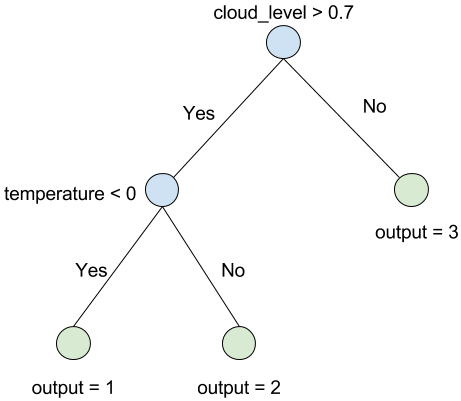
\includegraphics[height=3.0in]{sample_decision_tree}
  \caption{This is a decision tree model that could be used to predict whether the
  weather will be snowy (output 1), rainy (output 2), or neither (output 3) by
  looking at the cloud cover and temperature. The tree first checks if the cloud cover
  is high. If not, then it predicts there will be neither rain nor snow. Otherwise, the
  tree checks if the temperature is below 0. If so, then it predicts snow. Otherwise, it
  predicts rain.}
  \label{fig:sample_decision_tree}
\end{figure}

Random forest models and gradient boosted tree models are both ensembles of decision trees. They just differ in how they
are trained and applied. A random forest model trains many trees in parallel, where each tree is trained on a different bootstrapped
sample of the original dataset and where each split is only allowed to consider a subset of the features. A gradient boosted tree model
trains decision trees iteratively, where each successive decision tree learns to correct the mistakes of the previous trees. Like decision
trees, random forest and gradient boosted tree models can be used for both classification and regression. \cite{introtostatlearn}

These are not the only linear and tree models that are used in practice, but they are models that are supported in Spark.ML. 
Therefore, ModelDB S+C provides additional functionalty for the aforementioned models.

\section{Spark.ML}
Apache Spark \cite{spark} is a cluster computing engine that efficiently performs distributed computation
on data stored in-memory on many different machines. It is built around 
an abstraction called the Resilient Distributed Dataset (RDD). An RDD represents a dataset, its lineage,
and its partitioning. By tracking a dataset's lineage, an RDD allows the dataset to be recreated if it is
lost, thus providing fault tolerance. By tracking the partitioning and lazily performing operations, Spark
uses RDDs to schedule operations intelligently and pipeline them for efficiency.

Spark includes a number of libraries, two of which are relevant for this thesis. The first is Spark SQL,
which builds an abstraction called a DataFrame on top of the RDD abstraction. A DataFrame is simply a table
of data with named, typed columns. The second library
is Spark.ML, which lets users build machine learning models using Spark. Spark.ML lets the user create Transformers
that take an input DataFrame and produce an output DataFrame. It lets users use Estimators, which accept hyperparameters
and a DataFrame and produce a resulting model, which is simply a Transformer. Finally, Spark.ML provides a number
of other classes to support common model building tasks like cross validation and making preprocessing pipelines.

ModelDB S+C is built on three primitives: Transformer, DataFrame, and TransformerSpec, which are all inspired
by Spark SQL and Spark.ML. Transformer and DataFrame match their Spark counterparts, but unlike a Spark Estimator, a 
TransformerSpec simply describes how to create a model, rather than containing the logic for actually training the model.
ModelDB S+C does not train models, so there is no need for it to have model training logic.

The three primitives above, when coupled with ModelDB S+C's Syncable Event abstraction, can express a wide range
of model building operations.

The ModelDB Spark Client is a library designed for Spark.ML. It allows the user to use their existing
Spark.ML code, and with a few minor changes, store all their operations and models in ModelDB Server. 

\section{Machine Learning Libraries}
Since ModelDB Server aims to be library agnostic, it is worth looking at some other popular
machine learning libraries and understanding their abstractions for the model building process.

\subsection{MLI}
MLI \cite{mli} is an API for distributed machine learning. It includes an MLTable abstraction
that is very similar to the DataFrame abstraction in ModelDB S+C. MLI includes two other
tabular abstractions, the LocalMatrix and MLNumericTable, which are more restrictive forms of the
MLTable. MLNumericTable and LocalMatrix make computation easier, but they do not add anything to
the expressive power of MLI.

MLI's Optimizer and Algorithm abstractions help specify the logic for training a model. However,
as stated before, ModelDB S+C does not perform any training of models and thus these abstractions
are not important in the context of ModelDB S+C. That being said, the user can store information
about the algorithms and optimizer used to train a model in the hyperparameters of the model's associated
TransformerSpec.

MLI's Model abstraction maps to the Transformer abstraction in ModelDB S+C. There are two 
key differences between these abstractions. First, a Transformer is more general 
than a Model; it can represent data preprocessors as well as models. Second, a Model
stores the logic for making predictions while a Transformer does not. This is because
ModelDB S+C does not aim to make predictions, just to store and analyze the model building process. However,
the user is able to store serialized models in ModelDB S+C, which can later be deserialized and used to make
predictions.

\subsection{Scikit-learn}
Scikit-learn \cite{scikitlearn} is a machine learning library for Python. It expects data to
be given as matrices (two dimensional arrays in the numpy Python library) and DataFrames (from the Python
Pandas library). Both of these abstractions map nicely to ModelDB S+C's DataFrame.
A matrix can be thought of as a DataFrame where all columns are numeric and where the column names are ignored.

Scikit-learn includes the concept of an Estimator, which contains logic for training a model and stores the hyperparameters.
This maps well to ModelDB S+C's TransformerSpec. The logic for training the model is not necessary for ModelDB S+C. Scikit-learn
also includes Transformer and Predictor concepts. The former is almost identical to ModelDB S+C's Transformer abstraction while the 
latter is simply a more restrictive kind of Transformer.

Finally, Scikit-learn includes abstractions for cross validation and pipelines, much like Spark.ML does. Both of these
model building tasks are represented in ModelDB S+C as Syncable Events.

\subsection{Weka}
Weka \cite{weka} is a machine learning toolkit that includes a user interface targeted for non-expert users.
It represents data as tables, which is very similar to ModelDB S+C's DataFrame.
However, Weka does not include separate abstractions for describing a model and describing the fitting of a model. Instead,
it combines them together in an abstraction called a Scheme. Thus, ModelDB S+C's TransformerSpec and Transformer abstraction
together reflect the same information as a Weka Scheme. Finally, Weka includes pre-processing and post-processing utilities which
map well to ModelDB S+C's Transformer abstraction.

\subsection{Pylearn 2}
Pylearn 2 \cite{pylearn2} is a machine learning library geared towards researchers. It includes the concept of a Dataset, Model,
and TrainingAlgorithm, which are analogous to ModelDB S+C's concepts of a DataFrame, Transformer, and TransformerSpec.
ModelDB S+C's Transformer abstraction is more general than a Model because it can capture both models as well as data preprocessors.
Pylearn 2 also includes abstractions such as Cost and TerminationCriterion. Since ModelDB S+C does not concern itself with the
details of training models, it has no corresponding abstractions and instead allows the data scientist to specify cost and termination criterion
as hyperparameters in a TransformerSpec.

\subsection{Tensorflow}
Tensorflow \cite{tensorflow} is machine learning library that allows users to specify computation graphs, which is
especially useful for training neural network models. It represents data in the form of a Tensor. 
This is actually more general than the DataFrame concept in ModelDB S+C. However, using a tensor abstraction in ModelDB S+C may
add a good deal of complexity to the other abstractions without enabling a great deal of new functionality. 

Tensorflow represents data in the form of a computation graph, where nodes 
called variables use operations along edges to send tensors through the graph.
ModelDB S+C stores a graph, specified by the TransformEvents, where the 
nodes are DataFrames and the edges are Transformers. Tensorflow's computation 
graph is useful for performing efficient training of models. However, since 
ModelDB S+C does not actually do any training of models and instead just 
captures operations like transformations and model-fitting, its graph is 
different than TensorFlow's. Additionally, Tensorflow requires the user to 
specifiy their computation graph up-front in order for
the library to determine how to train the model. ModelDB S+C, on 
the other hand, builds up its graph over time as the user performs operations.

\subsection{Summary}
Thus, ModelDB S+C's abstractions seem to be general enough that there are analogs
in a number of other machine learning libraries. Of the examples above, Tensorflow
is the only one with a significantly different set of abstractions than ModelDB S+C.

\section{Model Building Support Systems}
ModelDB S+C does not actually train any machine learning models and it does not 
make any predictions. Rather, it collects, stores, and analyzes data about 
the model building process. In this way, ModelDB S+C supports the process of
model building rather than performing the process itself. This section describes
other systems that support the model building process.

\subsection{ModelHub}
ModelHub \cite{modelhub} is similar to the overall ModelDB system in that it also
aims to provide a suite of systems like model version control, a command line
toolkit, and a model exploration API, to support the model building process. ModelHub
focuses on deep learning and provides specialized tools for that domain, however, 
while ModelDB is aimed at machine learning models in general. Additionally, while
ModelHub tracks changes made to models, it does not track transformations 
made to datasets like ModelDB S+C does. Finally, ModelHub does not describe
any client libraries or abstractions that allow collecting data about the data
scientist's operations as they are performed. ModelDB Spark Client, on the other hand,
records a wide range of machine learning operations, like random splitting of datasets,
annotating datasets, and creating preprocessing pipelines, as the user does them and
stores them in ModelDB Server.

\subsection{MLDB}
MLDB \cite{mldb} is a system that allows users to create and store machine learning
models as well as datasets in a central database and access them through a REST API. 
While it supports the storage of models, it does not store operations (e.g. random splitting,
pipeline creation) that the user performs. Additionally, there are no client libraries
that can record these operations behind the scenes and send them to the server with
minimal user involvement. Finally, MLDB does not offer an API for querying operations
and gleaning information from them.

\subsection{Azure ML}
Microsoft's Azure Machine Learning \cite{azureml} is a cloud service that allows users
to create machine learning models with a web interface, store them in the cloud, and
access them via web service. Azure Machine Learning requires users to construct a dataflow 
graph indicating their full pre-processing and model training operations before model building
happens. ModelDB S+C, on the other hand, does not ask the user to indicate their full model building
workflow beforehand, and will instead record the operations and models as they appear. ModelDB Server
focuses on storing and analyzing the model building process and allows the user to use another library
(Spark.ML in this thesis) for training models. Azure Machine Learning, on the other hand, requires
that the user use its model training system. Finally ModelDB Spark Client works with a user's existing
Spark.ML code, allowing them to log their operations and models with few code changes. Azure Machine
Learning, on the other hand, requires users to convert significant parts of their code into
dataflow graphs using its proprietary user interface.

\subsection{Velox}
Velox \cite{velox} is a system for low latency serving and management of machine learning models.
While it does support storage of models, it does not store operations performed in model building and it
does not expose APIs for analyzing the model building process.

\subsection{MLBase}
MLBase \cite{mlbase} is a database system with the ability to store and serve machine learning
models. It includes an optimizer that figures out a plan for training a model. Unlike ModelDB S+C,
it does not track and store the operations in the model building process. It also requires users to
specify their model building process using a declarative language with hints for the optimizer. While this
can be useful for non-experts, it reduces the control that a user has over their model building process.
ModelDB S+C on the other hand, only requires a few minor changes to the user's Spark.ML code in order to
store the data associated with the model building process.

\subsection{PMML}
PMML \cite{pmml} is an XML-like markup language for representing machine learning models. While it
can describe a wide range of machine learning models, it cannot represent general model building operations
like ModelDB Server's database does. It is not possible to run queries on PMML either. ModelDB Server, on the other hand,
exposes an API for querying model building operations and stores operation data in a SQL database. PMML can,
however, complement ModelDB Server because a user can choose to store their serialized models in PMML form.

\subsection{Longview}
Longview is a predictive DBMS. It allows users to store machine learning models in a relational database
and access them via a user defined function in their queries. Unlike ModelDB S+C, it
cannot work with a user's existing code, and instead requires them to use Longview for all their
model training. Finally, Longview does not store machine learning operations like ModelDB Server does.

\chapter{Abstractions}

\section{Primitives}

\section{Syncable Events}

\section{Core Events}

\section{Composite Events}

\section{Specific Models}

\section{ModelDB Syncer}

\chapter{Algorithms}
The abstractions discussed in the previous chapter are stored in SQL tables in
ModelDB Server's database. This database is useful on its own because the user can
query it or build applications on top of it. Nevertheless, ModelDB Server provides
a number of algorithms that can be run on the database to glean useful information
about the model building process.

This chapter covers some of the algorithms used in ModelDB Server. 

The first section discusses storage algorithms, which describe how operations are stored in the database while
respecting the constraints between events and primitives. It begins by discussing the
storage algorithms for the three primitives and core
Syncable Events. Then, the storage algorithms for some
of the more complicated Syncable Events, such as RandomSplitEvent, GridSearchCrossValidationEvent,
and PipelineEvent are discuseed. Finally, the storage algorithms for linear and tree models are
covered.

The second section covers algorithms that operate on the DataFrame ancestry forest, which consists
of the DataFrames and the links between them, as reflected in the TransformEvents. The section explains
how the forest can be used to find the ancestry of a given DataFrame or model, the common ancestor of two
DataFrames, and the models that derived from a given DataFrame. The section concludes by showing how the
forest can be used to extract machine learning pipelines from ModelDB Server.

The third section focuses on algorithms that operate on the feature-sets of models. It first discusses how
it is possible to find the original DataFrame columns that were used to generate the features used by a given model.
Next, it explains how to find models that use all the features in a given feature set. 

The fourth section discusses algorithms that operate on multiple models. It begins by
discussing how the feature-sets of two models can be compared. Next, it explains
how the DataFrame ancestry forest can be used to find a common DataFrame from
which two models are derived. Afterwards, it shows how the hyperparameters of two
models can be compared. The section concludes by explaining how models can be ranked
and how ModelDB S+C can find models similar to a given model.

The fifth section focuses on algorithms for linear and tree models. It explains
how features can be ordered by importance, how models can be compared by convergence time,
and how feature importance can be compared between models.

The final section briefly mentions some other algorithms that ModelDB S+C provides, but which,
for brevity, are not covered at length in this thesis document.

\section{Storage Algorithms}
Before discussing the algorithms that glean information about model building, it
is important to first consider the algorithms that store data in ModelDB Server's 
database. These algorithms are straightforward, but it is illustrative to see
how they store data and what tables they affect.

\subsection{DataFrame, Transformer, and TransformerSpec}
To begin, consider the algorithms for storing the three primitives: DataFrame, 
Transformer, and TransformerSpec.

When ModelDB Server is asked to store a primitive, it first checks if there is already
a primitive in the database with the same ID. If not, then ModelDB Server stores the primitive
in the corresponding table. Next, it stores any auxiliary data (e.g. DataFrameColumns for a DataFrame, 
HyperParameters for a TransformerSpec) associated with the primitive.

\subsection{TransformEvent, FitEvent, MetricEvent}
The core Syncable Events are TransformEvent, FitEvent, and MetricEvent. They
are defined as compositions of the three primitives. Similarly, the algorithms
that store the core Syncable Events to the database utilize the storage algorithms
for the primitive events.

Consider the TransformEvent. When ModelDB Server is asked to store a TransformEvent, it
first stores the input DataFrame, output DataFrame, and Transforer using the corresponding
storage algorithm for the primitive. Then, it performs some processing specific to
TransformEvent (e.g. sorting and de-duplicating the input and output columns). Next,
it stores an entry in TransformEvent. Finally, it stores an entry in the Event table.

FitEvent and MetricEvent have storage algorithms that are similar in structure to TransformEvent's
storage algorithm.

\subsection{Annotation}
In order to store an Annotation, the client sends ModelDB Server a list containing 
the annotation fragments (each is a Transformer, TransformerSpec, DataFrame, or a String).
ModelDB Server first stores the primitives that the fragments refer to. Then, it stores
an entry in Annotation. Next, it stores an AnnotationFragment for each fragment. Finally,
it makes an entry in the Event table. ModelDB Server also verifies that each fragment refer
to exactly one primitive or contain a String. This check could also potentially be done at the database level.

\subsection{RandomSplitEvent}
This is a Syncable Event which represents the random splitting of a DataFrame
to create smaller DataFrames according to a weight vector. For example, doing
a random split of a 100-row DataFrame with weights of 0.7 and 0.3 would produce
DataFrames with row-counts of 70 and 30.

To store a RandomSplitEvent, ModelDB Server first makes an entry in a table
called RandomSplitEvent and an entry in Event. Next, it stores the input DataFrame
as well as all the output DataFrames. Then, it indicates the weight of each output
DataFrame in a table called DataFrameSplit. Finally, it stores TransformEvents to
indicate that the output DataFrames were derived from the input DataFrame (it uses
a synthetic Transformer called "RandomSplitTransformer" to reflect this operation).

Note that RandomSplitEvent demonstrates how to overcome TransformEvent's single-input,
single-output limitation. A RandomSplitEvent has a single input and multiple outputs.

\subsection{PipelineEvent}
Recall that PipelineEvent represents the creation of a Pipeline Model from a Pipeline.
A Pipeline is a chain of Transformers and Estimators (i.e. an object that applies a TransformerSpec
to a DataFrame create a Transformer). When a DataFrame is fed into the Pipeline, a Pipeline Model (a
chain of Transformers) is produced.  The storage algorithm is shown below:

\begin{algorithm}[H]
 \KwData{A PipelineEvent, denoted $pe$}
 Store $pe.pipelineFitEvent$, which stores the actual FitEvent that created the
 PipelineModel from the input DataFrame using a dummy Pipeline TransformerSpec.

 Sort $pe.transformStages$ and $pe.fitStages$ by stageNumber.

 Apply the merge procedure (i.e. from merge sort) to order all the stages by
 increasing stageNumber. Also require that a fit stage precede a transform stage
 if they have the same stageNumber.

 $currentDataFrame \gets pe.inputDataFrame$ 

 \For{each $stage$ in increasing stageNumber} {
   \eIf{$stage$ is a fit stage} {
     Store a FitEvent for the stage where $currentDataFrame$ is the the input DataFrame
     for the FitEvent.

     $currentDataFrame \gets stage.inputDataFrame$
   } {
     Store a TransformEvent for the stage where $currentDataFrame$ is the input DataFrame
     for the TransformEvent.

     $currentDataFrame \gets stage.outputDataFrame$
   }
 }

 \For{$fitStage$ in $pe.fitStages$} {
   Store an entry in the PipelineStage table.
 }

 \For{$transformStage$ in $pe.transformStages$} {
   Store an entry in the PipelineStage table.
 }

 \caption{Storage of a PipelineEvent}
\end{algorithm}

The key challenge in the PipelineEvent algorithm is enforcing the constraint that
the output of one pipeline stage is the input to the next pipeline stage. This is
done by processing the stages in increasing stageNumber (with fit stages put before
transform stages if they have equal stageNumbers). The $currentDataFrame$ variable
marks the input into the next pipeline stage.

\subsection{CrossValidationEvent}
Recall that a CrossValidationEvent corresponds to a single hyperparameter configuration.

To store a CrossValidationEvent, ModelDB Server first stores the input DataFrame and the
TransformerSpec (i.e. the hyperparameter configuration under consideration). Then, it
stores an entry in the CrossValidationEvent table and an entry in the Event table. Next,
ModelDB Server iterates through each fold in cross validation and, for each fold, it 
stores a FitEvent, MetricEvent, and an entry in CrossValidationFold. ModelDB Server also
enforces that the same input DataFrame is used for all the folds.

\subsection{GridSearchCrossValidationEvent}
Recall that grid search cross validation considers multiple hyperparameter configurations and
performs cross validation event for each one. GridSearchCrossValidationEvent's storage
algorithm is the following. First, a FitEvent is stored that represents the creation of
the final model over all the data. Next, an entry is made into the GridSearchCrossValidationEvent
table and an entry is made into the Event table. Then, all the DataFrames used for validation
and all the DataFrames used for training are stored, and a TransformEvent is logged for each to indicate
that they originated from the original input DataFrame. Next, the CrossValidationEvent storage algorithm
is run for each cross validation that was performed. ModelDB Server includes some additional logic to
ensure that the validation DataFrames and training DataFrames are shared across the different cross validations.

\subsection{LinearModel}
Recall that ModelDB S+C can augment the Transformer table with tables to store the
weights of a linear model. To store a linear model, ModelDB Server requires that the user
indicate (via ID) an existing Transformer to augment. Next, ModelDB Server makes an 
entry in the LinearModel table for the linear model. It then
stores a LinearModelTerm for each coefficient of the linear model. Next, it updates the Feature rows
associated with the Transformer with the feature importance scores computed by the linear model. Finally,
ModelDB Server logs the history of the objective function used for training into a table called ObjectiveFunctionHistory.

\subsection{TreeModel}
Recall that ModelDB S+C can augment the Transformer table with tables to store
ensembles of trees. In addition, recall that a decision tree model can be thought of
as an ensemble of one tree. 

The storage algorithm for a tree model goes as follows. First, ModelDB Server requires
the user to indicate (via ID) an existing Transformer to augment. ModelDB makes an entry in the TreeModel
table for the tree model. Then, for each tree in the model, ModelDB Server stores an entry in the TreeModelComponent table, 
then does a breadth first search starting
at the root for the tree, and for each encountered node, it stores an entry in TreeNode and (if the 
node is not the root node) an entry in TreeLink. Finally, after storing all the trees in the tree model, ModelDB Server
updates the Feature rows of the associated Transformer to indicate their feature importance scores as computed by the tree model.

\section{Ancestry Algorithms}
Recall that a TransformEvent indicates an input DataFrame and an output DataFrame. If each DataFrame is a node,
and there is a directed edge from input DataFrame to output DataFrame, then the TransformEvent table defines
a forest over all the DataFrames. This forest is hereafter referred to as the "DataFrame Ancestry Forest", or $\mathcal{F}$.
Suppose that each DataFrame, $df$, in $\mathcal{F}$ has a field $df.parent$ that points to the DataFrame that created it
and suppose that it also has a field $df.children$ that points to a list of the DataFrames that it produced.

There are a number of interesting algorithms that can be run on $\mathcal{F}$.

\subsection{Ancestry of a DataFrame}
The simplest algorithm is to find the ancestry of a DataFrame. That is, given a DataFrame $df$ in $\mathcal{F}$, we
follow parent pointers all the way up to a root DataFrame (i.e. a DataFrame with an empty parent pointer). The reverse
of this path is the ancestry of a given DataFrame. This operation allows a data scientist to see how a particular DataFrame
was created and identify where potential bugs in the data may have been introduced.

\subsection{Ancestry of a Model}
It is also possible to find the ancestry of a model. Recall that a model is simply a Transformer with an associated
FitEvent. Finding the ancestry of a model involves looking up the DataFrame in its associated FitEvent and finding the
ancestry of that DataFrame. This allows the user to see what DataFrames contributed towards the data used to train a model.

\subsection{Common Ancestor of Two DataFrames}
Given two DataFrames $df1$ and $df2$ in $\mathcal{F}$, it is possible to find the common ancestor DataFrame (if there is one)
that led to their creation. This can be useful in finding commonalities between intermediate DataFrames (e.g. $df1$ is producing
good results and $df2$ is producing bad results - where in their lineage did they start to differ?). Finding the common ancestor
is implemented by simplying finding the ancestry of $df1$ and the ancestry of $df2$, and finding youngest DataFrame common to both
the ancestries.

\subsection{Descendent Models of DataFrame}
In addition to following parent pointers in $\mathcal{F}$, it is also useful to follow child pointers. A data scientist
may be interested in determining all the models that used data that originated in a DataFrame $df$. To compute this,
a breadth-first search is performed starting at $df$ and following child pointers. All the DataFrames encountered in 
the search are added to a list $descendentDfs$. Then, a scan is made of the FitEvent table to find all Transformers that
were created by fitting a DataFrame in $descendentDfs$. These are the models that descended from $df$.

\subsection{Pipeline Extraction}
The user may explicitly create Pipeline Models via ModelDB S+C's PipelineEvent. However, since Pipeline Models are 
simply chains of Transformers (some of which were produced by fitting a TransformerSpec to a DataFrame),
the user implictly creates Pipeline Models as they make FitEvents and TransformEvents. ModelDB Server offers a mechanism
for extracting pipelines from $\mathcal{F}$. The algorithm for extracting a pipeline is specified below.

First the user specifies the ID, $mId$, of a model (i.e. Transformer with assocaited FitEvent) that they'd like to extract
a pipeline for.

Second, the FitEvent table is scanned to find the DataFrame $df$ that is associated with the Transformer with ID $mId$.

Third, the ancestry of $df$ is computed, and all the TransformEvents along the chain are noted down in a list (call it $transformEvents$).

Fourth, the Transformer for each TransformEvent in $transformEvents$ is extracted and put into a list (call it $transformers$).

Fifth, the FitEvent table is scanned and the TransformerSpec is extracted for all the FitEvents who have a Transformer appearing in $transformer$ 
(call the resulting list of TransformerSpecs $specs$).

Finally, $transformers$ and $specs$ are returned to the user, sorted by the position of their corresponding TransformEvent in the ancestry chain.

\section{Feature Algorithms}
The Feature table lists the features that are used by a model (i.e. Transformer with associated FitEvent).
There are a number of useful operations we can perform using this table.

\subsection{Original Feature-set of Model}
Suppose that there is a DataFrame $df1$ with the columns $labScore$ and $homeworkScore$. Then,
suppose that $df1$ is transformed to produce $df2$, which contains a column called $assignmentScore$ that is
computed by combining $labScore$ and $homeworkScore$ in some way. Finally, suppose that a model, $m$, is created to
predict a new column, called $finalExamScore$, based on the value of $assignmentScore$.

In the above example, $m$ has a single feature column, $assignmentScore$. However, the data scientist may find
it useful to find the original features that produced the $assignmentScore$ column (i.e. $labScore$ and $homeworkScore$).

It is possible to use the Feature table and the DataFrame ancestry forest ($\mathcal{F}$) to compute the original
features. The algorithm for doing so is presented below.

First, the user must specify the ID (call it $mId$) of a model.

Second, the corresponding FitEvent for model $mId$ is found, and its DataFrame (call it $df$) is extracted.

Third, a set called $originalFeatures$ is initialized to contain the features (from the Features table) of model $mId$.

Fourth, the ancestry of $df$ is computed, with the TransformEvents noted down in the list $transformEvents$.

Fifth, the $transformEvents$ list is scanned such that the TransformEvent that directly produced $df$ is first and the
TransformEvent that operated on a root DataFrame is last. For each such TransformEvent $transformEvent$, the following steps are
performed:
\begin{enumerate}
  \item If none of the columns listed in $originalFeatures$ appears 

    in $transformEvent.outputColumns$, then $transformEvent$ 

    is skipped and the next TransformEvent is considered.
  \item Otherwise, all the columns in $originalFeatures$ that are also 

    in $transformEvent.outputColumns$ are removed from $originalFeatures$.
  \item All columns in $transformEvent.inputColumns$ are added to $originalFeatures$.
\end{enumerate}

Finally, $originalFeatures$ is returned.

The above algorithm simply starts with the model's described feature columns and walks up the ancestry chain trying to find
the columns that originated these columns.

\subsection{Models using a Given Feature-set}
ModelDB Server can also find models that use any of the features listed in a given set of features, $featureSet$. Basically,
the Feature table is scanned for rows whose feature name is included in $featureSet$. The Transformer IDs for these
Feature rows are extracted, de-duplicated, and returned to the user.

Note that a data scientist may find it useful to find all the models that indirectly OR directly use any features in a 
given feature set. The above algorithm handles the "directly" case, but a variation of the Original Features algorithm would
be needed to handle the "indirectly" case. This has not been implemented, but may be a useful algorithm to implement in the future.

\section{Multi-model Algorithms}
A data scientist creates multiple models in the model building process, and therefore may want
to compare models in some way to help select the best ones. The algorithms
described in this section offer some useful ways of doing this.

\subsection{Compare Features of Two Models}
One simple operation is to find the features shared by two models. Given the IDs
of two models, $mId1$ and $mId2$, ModelDB Server finds their corresponding features 
(by scanning the Feature table) and returns the features they have in common, 
as well as the features that appear in only one of them.

While it has not been implemented, it would not be hard to utilize the Original Features algorithm here
so that the original, rather than direct, features of the models are compared.

\subsection{Common Ancestor DataFrame of Two Models}
Identifying the DataFrame from which two models are derived can be useful in
understanding their commonalities. Given the IDs, call them $mId1$ and $mid2$, 
of two models, ModelDB Server finds the common ancestor DataFrame as follows.

First, the FitEvent table is scanned to yield the DataFrames $df1$ and $df2$
that produced the models with IDs $mId1$ and $mId2$.

Then, the common ancestor DataFrame (using the algorithm described earlier in
this chapter) of $df1$ and $df2$ is computed and returned.

\subsection{Compare Hyperparameters of Two Models}
Models of the same type (e.g. Random Forest) can have wildly different performance
outcomes on the same training DataFrame because they have different hyperparameters.
ModelDB Server makes it possible to compare the hyperparameters of two models given their
IDs (call them $mId1$ and $mId2$).

First, the FitEvents for $mId1$ and $mid2$ are read and their TransformerSpecs $spec1$ and
$spec2$, respectively, are extracted.

Second, the hyperparameters for $spec1$ and $spec2$ are read from the HyperParameter table
and put into lists $hyperparameters1$ and $hyperparameters2$, respectively,

Third, hyperparameters in $hyperparameters1$ and $hyperparameters2$ with the same name are
extracted and put into a list called $commonHyperparameters$. Hyperparameters with names unique to just
one of lists are put into lists called 

$model1Hyperparameters$ and $model2Hyperparameters$.

Finally, the three resulting hyperparameter lists are
returned to the user.

\subsection{Rank Models}
Sometimes, a user may want to find the model that performs best in a given set of
models. Since ModelDB Server stores MetricEvents for these models, it can sort the models
according to a given metric type (e.g. accuracy) when evaluated on a given DataFrame.

\subsection{Find Similar Models}
A user may want to find other models similar to a given model. ModelDB Server
allows the user to do search for models that match the given model's type (e.g. 
Random Forest), problem type (e.g. regression, binary classification), performance,
and more.

\section{Linear Model and Tree Model Algorithms}
ModelDB S+C stores extra data about linear and tree models, and this section 
summarizes a few of the algorithms that can be run on these models.

\subsection{Features ordered by Importance}
One operation of great value in model building is computing the most important
features in a model. ModelDB Server stores an importance column in the Feature
vector for its linear and tree models. Thus, it simply sorts the features in
descending importance and returns them to the user.

For linear models, ModelDB Server only computes feature importance if the linear model
is standardized (i.e. all feature columns were scaled to have zero mean and unit variance).
In this case, the feature importance is taken to be the absolute value of the weight 
associated with the feature.

For tree models, ModelDB Server defers to Spark.ML's implementation of feature importance. Thus,
the Spark Client uses Spark.ML's algorithm to compute feature importances and then notifies 
ModelDB Server. However, since ModelDB Server stores the entire tree model in its database, this algorithm
could also just be implemented in ModelDB Server directly.

\subsection{Iterations Until Convergence}
ModelDB Server has a table called ObjectiveFunctionHistory, which stores, for a given model,
the value of the objective function over several iterations of training. With this table in hand,
it is easy for ModelDB Server to simply return the number of iterations taken for a model to converge
(convergence occurs when the value of the objective function changes by less than $\epsilon$ in a single
iteration).

\subsection{Compare Feature Importances}
ModelDB Server also supports comparing the importance of features between two models. First, it gets
the list of features for each model, ordered by importance. Using the order, it then computes the
percentile ranking of the feature's importance. Then, ModelDB Server finds features common to both features
and returns the percentile ranking of the feature in each model. It also returns the percentile rankings for
the features that appear in only one of the models.

\section{Other Algorithms}
There are a number other algorithms that ModelDB Server supports (e.g. building confidence intervals
for linear model coefficients) and even more that can be implemented without much code (e.g. for a given model, see if there is another
model that has scored higher than it for every MetricEvent). For brevity, however, these algorithms will not be discussed.

\chapter{Implementation}
This chapter discusses some important aspects of ModelDB S+C's implementation.

\section{System Architecture}
The overall architecture for ModelDB S+C is shown below in Figure 
\ref{fig:system_architecture}.

\begin{figure}
  \centering
  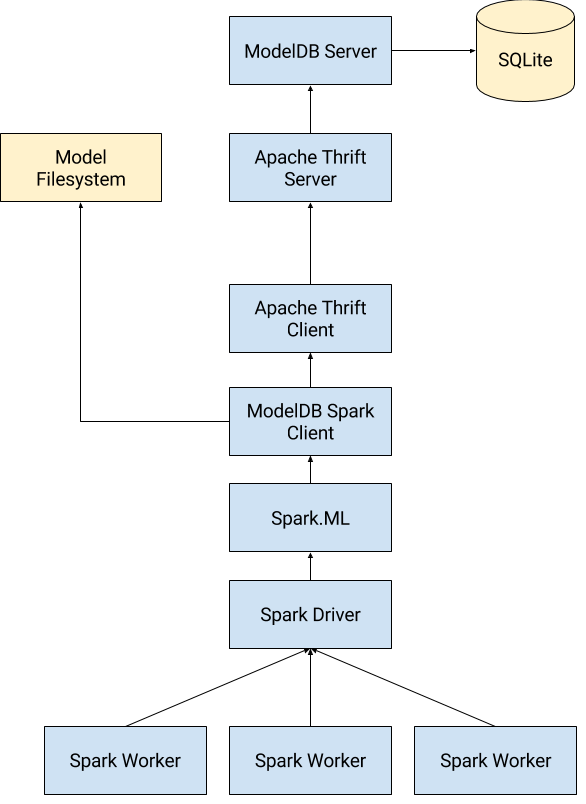
\includegraphics[height=4.0in]{system_architecture}
  \caption{
    The overall architecture of ModelDB S+C. The arrows indicates the flow
    of operations + models data. Notice that the data originates at the Spark workers and
    finds its way into the SQLite database or model filesystem.
  }
  \label{fig:system_architecture}
\end{figure}

In the figure, the operations occur and the models first appear on the Spark worker nodes.
These nodes send their data to the Spark driver node. The driver node runs the Spark.ML
library, which stores objects representing the models and which has functions to trigger
the operations. The ModelDB Spark Client sits on top of the Spark.ML library, and receives the
operations and model data. The Spark Client runs an Apache Thrift client, which it uses to
send data to ModelDB Server. ModelDB Server receives the data, performs the appropriate computations,
and stores it in the SQLite Database. Notice that ModelDB Server does not speak directly to the
model filesystem, which contains the serialized model files. Instead, the Spark Client speaks directly
to the model filesystem. The reasoning for this decision will be discussed later in this chapter.

Recall that ModelDB Server also exposes an API for gleaning information about the model building process.
Spark Client includes convenience functions that the user can call to get this information. In this case,
the arrows would be reversed. When the Spark Client makes a request (via Apache Thrift) to ModelDB Server to run an API 
method, ModelDB Server reads the database, performs the appropriate computations, and responds to the Spark Client. The
Spark Client then extracts the desired information from the response, and returns it to be used in user's driver node
program.

The two key pieces of this diagram are the ModelDB Server and Spark Client. Both
will be discussed below.

\section{Server}
While there is a good deal of code (written in Java) in ModelDB Server, this section will focus only
on interesting pieces of implementation that were not described in the previous chapters.

\subsection{Database}
Currently, ModelDB Server stores its data in a SQLite database. However, it can be
configured to use a number of other SQL databases, like PostgreSQL. This is primarily
achieved by using the JOOQ library. This library asks the user to provide a configuration
file that specifies the database and runs a code generator to create Java classes that
ModelDB Server can use to interact with the database. Changing this configuration file
(and making appropriate changes to the database schema, in order to correct for slight differences
in SQL between languages) can allow ModelDB Server to use a different SQL database than
SQLite. In addition, ModelDB Server is designed to avoid using any esoteric SQLite data types,
functions, or features. Some problems which could be solved by appealing to to a special 
database function are instead solved in ModelDB Server. This places minimal requirements on 
the SQL database that ModelDB Server uses.

\subsection{Model Filesystem}
ModelDB Server allows the user to store their serialized model files in a filesystem. However,
as shown in \ref{fig:system_architecture}, the ModelDB Server does not ever communicate with this
filesystem. Instead, the flow is as follows.

First, the user calls a function in ModelDB Spark Client to indicate that they'd like to save a model and optionally
provides a filename that they would like to use.

Second, the Spark Client indicates to the ModelDB Server that it would like to store the given model under the
given filena,e.

Third, ModelDB Server generates a filepath (incorporating the user's requested filename, if one is provied)
for the model, updates the model's entry in Transformer table 
to reflect this filepath, and sends the filepath to the Spark Client.

Finally, the Spark Client serializes the model and writes the result to the designated filepath.

There are a number of advantages that the above approach has over an approach in which the client
sends the serialized model to the server and the server stores the model in the filesystem. First,
the serialized model file may be large, so storing it directly to the filesystem is cheaper than
first sending it to the server and having the server store the model. Second, some machine learning
libraries (e.g. Spark.ML) store models in a directory structure rather than as a file, and having the
client store the model directly to the given filepath makes this possible. Finally, by pushing the storage
logic to the client, the client could allow the user to provide logic that stores a serialized model
to a completely different filesystem (perhaps their own experimental filesystem). 

\subsection{Configuration}
All the configuration for ModelDB Server (e.g. port to launch server on, prefix for
filepath generation) is defined in a single configuration file, and some sensible defaults
are provided so that ModelDB Server is usuable right out of the box rather than requiring
configuration before use.

\subsection{Stateless, Separated, Logic}
ModelDB Server exposes all its functionality to the client as Thrift endpoints. The client
can make remote procedure calls to this endpoint to store operations, store models, compute 
ancestries, and more. The actual implementation of these Thrift endpoints are extremely short,
most of them being just a single function call. This is done for three reasons. First, it
pushes all of ModelDB Server's logic into other classes, called Data Access Objects (DAOs), 
for which unit tests can be easily written without having to worry about complexities that 
come with using Apache Thrift. Second, it allows ModelDB Server to be used as a library, 
so that other programs could import and use it without having to launch a Thrift server. 
Finally, it makes the server stateless, which can be useful if
future work adds support to scale ModelDB Server to multiple servers.

The ModelDB Server algorithms described in Chapter 4 are each implemented as a single function
or group of functions. They do not persist state between executions and they are expect to have all
their dependencies injected as arguments. The abstractions described in Chapter 3 are implemented as 
SQL tables and also have corresponding Thrift structures to allow them to be sent and received via Thrift
calls.

\section{Spark Client}
The Spark Client is written in Scala, primarily because Spark is written in Java.
Before discussing the implementation details, it is worth seeing a sample usage
of the Spark Client.

\subsection{Sample Usage}
Consider the following sample code, written without ModelDB Spark Client, 
in which a model is trained and evaluated.

\begin{minted}{scala}
val Array(train, test) = data.randomSplit(Array(0.7, 0.3))
val lr = new LogisticRegression()
      .setMaxIter(20)
      .setLabelCol(FeatureVectorizer.indexed(labelCol))
      .setPredictionCol(predictionCol)
      .setFeaturesCol(featuresCol)
val ovr = new OneVsRest()
      .setClassifier(lr)
      .setLabelCol(FeatureVectorizer.indexed(labelCol))
      .setPredictionCol(predictionCol)
      .setFeaturesCol(featuresCol)
val model = ovr.fit(train)
val predictions = model.transform(test)
val eval = new MulticlassClassificationEvaluator()
      .setLabelCol(FeatureVectorizer.indexed(labelCol))
      .setPredictionCol(predictionCol)
      .setMetricName("f1")
val score = eval.evaluate(predictions, model)
\end{minted}

Below, consider the same code WITH ModelDB Spark Client. The changed or
new lines are commented.

\begin{minted}{scala}
// New line.
import edu.mit.csail.db.ml.modeldb.client.ModelDbSyncer._

// New line.
val syncer = ModelDbSyncer.setSyncer(new ModelDbSyncer())

// Use randomSplitSync instead of randomSplit.
val Array(train, test) = data.randomSplitSync(Array(0.7, 0.3))
val lr = new LogisticRegression()
      .setMaxIter(20)
      .setLabelCol(FeatureVectorizer.indexed(labelCol))
      .setPredictionCol(predictionCol)
      .setFeaturesCol(featuresCol)
val ovr = new OneVsRest()
      .setClassifier(lr)
      .setLabelCol(FeatureVectorizer.indexed(labelCol))
      .setPredictionCol(predictionCol)
      .setFeaturesCol(featuresCol)

// Use fitSync instead of fit.
val model = ovr.fitSync(train)

// Use transformSync instead of transform.
val predictions = model.transformSync(test)
val eval = new MulticlassClassificationEvaluator()
      .setLabelCol(FeatureVectorizer.indexed(labelCol))
      .setPredictionCol(predictionCol)
      .setMetricName("f1")

// Use evaluateSync instead of evaluate.
val score = eval.evaluateSync(predictions, model)
\end{minted}

As displayed above, the key changes required to use ModelDB Spark Client are to
import and set up the ModelDB Syncer (the first two lines) and append the suffix
"Sync" to the operations that the user would like to store in ModelDB Server. ModelDB
Spark Client provides "Sync" variants of many Spark.ML methods such as evaluate(),
transform(), fit(), save(), and randomSplit(). Additionally, the ModelDBSyncer
object (called "syncer" in the code sample above) exposes a number of methods for
interacting with ModelDB Server as well (e.g. deserialize a model stored on the
Server, compute ancestry of a DataFrame).

ModelDB Spark Client uses the same types as Spark.ML, so it should interact nicely
with other Spark.ML code and with other libraries that build on Spark.ML. Additionally,
it does not re-implement the functionality of Spark.ML, it only adds functionality. To
understand how this is done, it is worth looking at some aspects of the implementation.

\subsection{Syncable Event}
Recall that a Syncable Event represents an operation that can be stored on ModelDB Server.
The ModelDB Spark Client has a SyncableEvent class that is responsible for converting Spark objects
into their corresponding Thrift structures and then making the appropriate Thrift endpoint call to
store the operation and its primitives on ModelDB Server. Specifically, SyncableEvent is a class
from which many other subclasses derive. These subclasses implement a few methods:

\begin{enumerate}
  \item \textbf{constructor}: The constructor accepts a number of Spark.ML objects (e.g.
  a DataFrame, Estimator, and Transformer, in the case of FitEvent) and sets them as state variables.
  \item \textbf{makeEvent}: This method uses the state variables described above and
  creates a Thrift structure representing the event.
  \item \textbf{sync}: This method calls makeEvent and stores the result on ModelDB Server
  using the appropriate API endpoint. It then passes the result of the API call to the
  associate method.
  \item \textbf{associate}: This method uses the result of the API call to update the
  ModelDBSyncer as appropriate. This includes, for example, updating the ID mappings. The
  ModelDBSyncer is described later in this chapter.
\end{enumerate}

There are SyncableEvent subclasses for all of the Syncable Events that can be stored
on ModelDB Server. These include FitEvent, TransformEvent, MetricEvent, GridSearchCrossValidationEvent,
and more.

\subsection{ModelDBSyncer}
The Spark Client includes a global object called the ModelDBSyncer. This object has a few responsibilities:

\begin{enumerate}
  \item It maintains a buffer of SyncableEvents, which it periodically flushes (by calling sync() on each
  entry of the buffer). The user can configure the syncing strategy (e.g. sync immediately when the buffer contains
  a SyncableEvent, sync only when the ModelDBSyncer is explicitly told to sync).
  \item It exposes convenience functions for interacting with ModelDB Server's API endpoints
  for gleaning information about the model building process (e.g load a deserialized model,
  find the original features that were used to create a model).
  \item It maintains some state about the Spark objects. For example, it stores a mapping between
  Spark objects (e.g. Transformer) to their corresponding IDs in ModelDB Server. This makes it possible to easily get
  the Spark object with a given ID and to get the corresponding ID of a Spark object. Another example, it stores, for
  each DataFrame, the filepath containing the DataFrame's data.
  \item It implements all the traits in the ModelDB Syncer, making it possible to bring all the implicit classes
  into the user's program with just a single import statement.
\end{enumerate}

\subsection{Implicit Classes and Traits}
ModelDB Spark Client aims to augment methods in Spark.ML without having to reimplement or
modify any existing code in Spark.ML. For example, consider the following Spark.ML method:

\begin{minted}{scala}
val model = estimator.fit(dataframe)
\end{minted}

The above method call uses an Estimator to train a model (a Transformer) on a DataFrame.


ModelDB Spark Client includes the following method, which involves the same estimator, dataframe,
and model objects indicated above and each one is the same type as it is in the code sample above.

\begin{minted}{scala}
val model = estimator.fitSync(dataframe)
\end{minted}

This is almost identical in function to Spark.ML's fit method, except that it logs a FitEvent
(or a GridSearchCrossValidationEvent, PipelineEvent if estimator is a CrossValidator or Pipeline,
respectively) to ModelDB Server.

To make the above code possible, ModelDB Spark Client uses a combination of Scala implicit classes
and Scala traits. A Scala trait is similar to an interface in Java or C\#, but it also provide default
implementations for interface methods. A Scala implicit class serves a purpose similar to Java's autoboxing
and unboxing features.

Implementing the fitSync above requires the following:

\begin{enumerate}
\item A Scala trait called SyncableEstimator is defined.
\item Inside SyncableEstimator, a Scala implicit class for Estimator, called EstimatorSync,
is defined. This EstimatorSync implicit class contains an implementation for fitSync(), which calls fit()
on its corresponding Estimator object, creates a FitEvent (a SyncableEvent in Spark Client), and buffers it
onto the global ModelDBSyncer.
\item ModelDBSyncer is marked as implementing the SyncableEstimator trait, so that the EstimatorSync implicit class
is automatically imported into the user's main program. 
\end{enumerate}

Thus, when the user calls fitSync, the following occurs.

\begin{enumerate}
\item Scala looks for an implementation of fitSync() in the Estimator class, and cannot find one.
\item Scala notices there is an implicit class (imported when ModelDBSyncer was imported) 
for Estimator called EstimatorSync that does implement fitSync().
\item Scala creates an EstimatorSync object and passes the Estimator object as a constructor argument.
\item Scala calls the fitSync() method on the EstimatorSync object.
\item Scala returns the result of the fitSync() call, which is the trained model.
\end{enumerate}

This makes it possible augment the Estimator class's fit() function so that it 
buffers a FitEvent in the ModelDBSyncer without having to rewrite or edit existing Spark.ML code.

This technique is used many times in ModelDB Spark Client (e.g. for transformSync(), evaluateSync()).

\subsection{FeatureVectorizer}

ModelDB Spark Client also includes a class called FeatureVectorizer which is a convenience class
for building pre-processing pipelines. The user specifies a DataFrame and indicates the categorical and numerical columns
they'd like to use. Then, FeatureVectorizer builds a PipelineModel that performs common preprocessing steps (e.g. string indexing,
one-hot encoding, standardization of numerical columns) and creates an output DataFrame with a "features" column that can
be used by a machine learning Estimator or Model.


\chapter{Evaluation}
By importing ModelDBSyncer and appending "Sync" to the method names, the user
can use ModelDB Spark Client to record and send their operations and models
on ModelDB Server, which stores the data in its database and model filesystem.
Naturally, this takes extra running time and storage space than if the user did
not use ModelDB S+C at all. Additionally, the API methods exposed by ModelDB Server
take some time to run too. The goal of this chapter is to measure whether the time
and space requirements of ModelDB S+C are reasonable.


\section{Overview}
Experiments were conducted to answer the following questions:

\begin{enumerate}
\item Is the time overhead of storing operations and models on ModelDB Server reasonably small (compared to
the overall running time of the Spark.ML program)?
\item Is the space taken up by ModelDB S+C's database and model files reasonably small (compared
to the size of the dataset)?
\item Are ModelDB S+C's tree model and linear model representations reasonably small (compared 
to the size of corresponding PMML files)?
\item Is the time take to execute the ModelDB Server API methods reasonably small (compared
to the training time of the model)?
\item Can ModelDB S+C record most of the machine learning operations in real Spark.ML programs?
\end{enumerate}

The chapter also discusses performance improvements that can further improve ModelDB S+C with
regard to the above questions.

\section{Datasets}
 \begin{table}
   \centering
    \begin{tabular}{ | l | l | l | l |}
      \hline
      Dataset Name & Problem Type & Number of Rows & Number of Features \\ \hline
      IMDB & Regression & 5,043 & 28 \\ \hline
      Animal Shelter & Multiclass Classification & 26,729 & 10 \\ \hline
      Housing Prices & Regression & 1,460 & 81 \\ \hline
      Iris & Multiclass Classification & 150 & 5 \\  \hline
      Titanic & Binary Classification & 1,309 & 14  \\  \hline
      SMS Spam & Binary Classification & 5,574 & N/A (text) \\  \hline
      Flight Delays & Binary Classification & 7,453,215 & 29 \\ 
      \hline
   \end{tabular}
   \caption{Datasets used in evaluation}
   \label{tab:datasets}
 \end{table}

ModelDB S+C was evaluated on real datasets, which are described below and outlined
in Table \ref{tab:datasets}.

The \textbf{IMDB} dataset \cite{imdb} includes features like genre, number of
reviews, language, and more for over 5000 movies in the IMDB Movie Database. The dataset
also includes the IMDB score (i.e. a 1 to 10 rating of how good the movie is considered)
for each movie. A machine learning model could solve a regression problem on this
dataset in which it predicts the IMDB score for a given movie. Such a model could
be used to identify the best movies and recommend them to users. This dataset
was used when measuring the time/space overhead of ModelDB S+C and was also used
when measuring the execution time for ModelDB Server API methods.

The \textbf{Animal Shelter} dataset \cite{animal} includes features like
animal type (cat or dog), breed, color, age, and more for over 25,000 animals. The
dataset also includes the animal's outcome (e.g. adopted, returned to owner, transferred)
for each animal. A machine learning model could solve a multi-class classification problem on this dataset
in which it predicts the most likely outcome for a given animal. Such a model could 
be used to identify the most likely outcome for an animal newly admitted into the
animal shelter. This dataset was used when measuring the time/space overhead
of ModelDB S+C.

The \textbf{Housing Prices} dataset \cite{housing} includes features like square
footage, number of bathrooms, neighborhood type, and more for about 1,500 houses.
The dataset also includes the sale price of each house. A machine learning model
could solve a regression problem on this dataset in which it predicts the sale
price of a given home. Such a model could be used by realtors who
are trying to find the best price for a home when putting it up on the market. This
dataset was used when measuring the time/space overhead of ModelDB S+C.

The \textbf{Iris} dataset \cite{iris} is a famous dataset that includes features
like petal length, sepal width, and more for 150 Iris plans. The dataset also
includes the species of the Iris plant. A machine learning model could solve a 
multi-class classification problem on this dataset in which it predicts the species
of a given Iris plant. Such a model may be useful for botanists looking to classify
their plants. This dataset was used when comparing the size of ModelDB S+C models
to PMML models (the PMML website includes model files for the Iris dataset).

The \textbf{Titanic} dataset \cite{titanic} is a famous dataset includes features like 
passenger sex, passenger class, and more for over 1300 passengers of the Titanic. 
The dataset also includes whether each passenger survived or died. A machine learning
model could solve a binary classification problem on this dataset in which it predicts whether
a given passenger survived. Such a model may be useful for historians. This dataset
was used when evaluating ModelDB S+C on an existing machine learning workflow.

The \textbf{SMS Spam} dataset \cite{spam} includes over 5500 text messages and
a label indicating whether the message is spam or not. A machine learning model
could solve a binary classification problem on this dataset in which it predicts
whether a given text message is spam. Such a model could be used as a text messaging
app's spam filter. This dataset was used when evaluating ModelDB S+C on an existing
machine learning workflow.

The \textbf{Flight Delays} dataset \cite{airline} includes features like carrier, departure
time, and more for over 7 million airplane departures. It also includes a field indicating whether
the plane was delayed. A machine learning model could solve a binary classification problem on this dataset in which
it predicts whether a given airplane is delayed. Such a model could be used by airports and airlines
to anticipate delays for particular airplanes. This dataset was used when evaluating ModelDB S+C
on an existing machine learning workflow.

\section{Methodology}
\subsection{Machine}
These experiments were run on a DigitalOcean machine with a 160 GB SSD disk, an 8 core processor,
and 16GB of memory.

\subsection{Time and Space Overhead}
The first experiment focused on evaluating the time and space overhead of ModelDB S+C.
The IMDB, Housing Prices, and Animal Shelter datasets were used for this experiment. 

First, for each of the datasets listed above, three programs (called workflows) were
created. The \textbf{simple} workflow simply trains and evaluates one machine learning model. 
The \textbf{full} workflow creates a preprocessing pipeline for the data, trains 
some models with grid search cross validation (thus trying many hyperparameter configurations), 
and evaluates the best model. The \textbf{exploratory} worklow executes many full workflows, 
trying different model types (e.g. random forest, linear regression) and different feature sets.

Second, a program was written to artificially increase the size of the dataset by duplicating rows.
Dataset sizes were varied from the dataset's original number of rows to one million rows.

Third, ModelDB Spark Client was instrumented so that it recorded the time spent running code related
to ModelDB S+C.

Fourth, each (dataset, dataset size, workflow) triple's program was executed with ModelDB S+C enabled. The time that ModelDB S+C spent
recording and storing each operation and model was recorded. The database size, number of rows in each table, and size of the model
files was also recorded. Finally, the overall running time of the program and the size of the (artificially enlarged) dataset
were also noted. Due to Spark's large memory requirements, it was not possible to run the exploratory workflow for the 
housing dataset when the number of rows was large because Spark.ML consumed too much memory. This is because Spark is designed
to be run on machines with large amounts of RAM, and the machine used for these experiments had only 16 GB of RAM.

\subsection{Computation Time of API Methods}
The second experiment focused on evaluating the running time of ModelDB Server's API methods. The
IMDB dataset was used here.

First, the IMDB exploratory workflow was run to populate ModelDB Server's database.

Second, the database was duplicated $N$ times (i.e. $N$ additional rows were created for
every row in every table of the database), where $N$ was varied from 0 to 400. This was
done to simulate many exploratory workflows being run on ModelDB S+C.

Third, various API methods were executed on the (artificially enlarged) database and the
running time for each method was recorded.

\subsection{Compare ModelDB S+C Models to PMML}
The PMML website \cite{pmmlwebsite} includes sample files for a 200 tree random forest model
and logistic regression model that were trained on the Iris dataset. So, this
experiment trained a 200 tree random forest model and a one vs. rest logistic regression model
in Spark.ML (with ModelDB S+C enabled). The sizes of the model files and database
were recorded.

\subsection{Evaluating Existing Workflows}
Three machine learning workflows were collected from the Internet. The first \cite{flightworkflow}, from
a Hortonworks article, uses the Flight Delays dataset to build a classification model to predict
delays. The second \cite{titanicworkflow} and third \cite{spamworkflow} are from ZeppelinHub, a website that allows users to share their
machine learning workflows as Zeppelin notebooks. The second workflow trains two models
to predict passenger survival status for the Titanic dataset and the third builds a spam classifier
using the SMS Spam dataset. These workflows were cleaned up, ported to Spark v2.0.0, and 
augmented with ModelDB Spark Client (i.e. import ModelDbSyncer and add *Sync to the methods).

\section{Time Overhead Results}
To measure the time overhead, the time spent running ModelDB S+C code is divided 
by the total running time of the program and the result is taken as a percentage.
Plotting this time overhead percentage, for each (dataset, workflow) pair,
as a function of the number of rows in the dataset yields Figure \ref{fig:time_overhead}.
For this experiment, ModelDB S+C did NOT count the number of rows in each DataFrame.

\begin{figure}
  \centering
  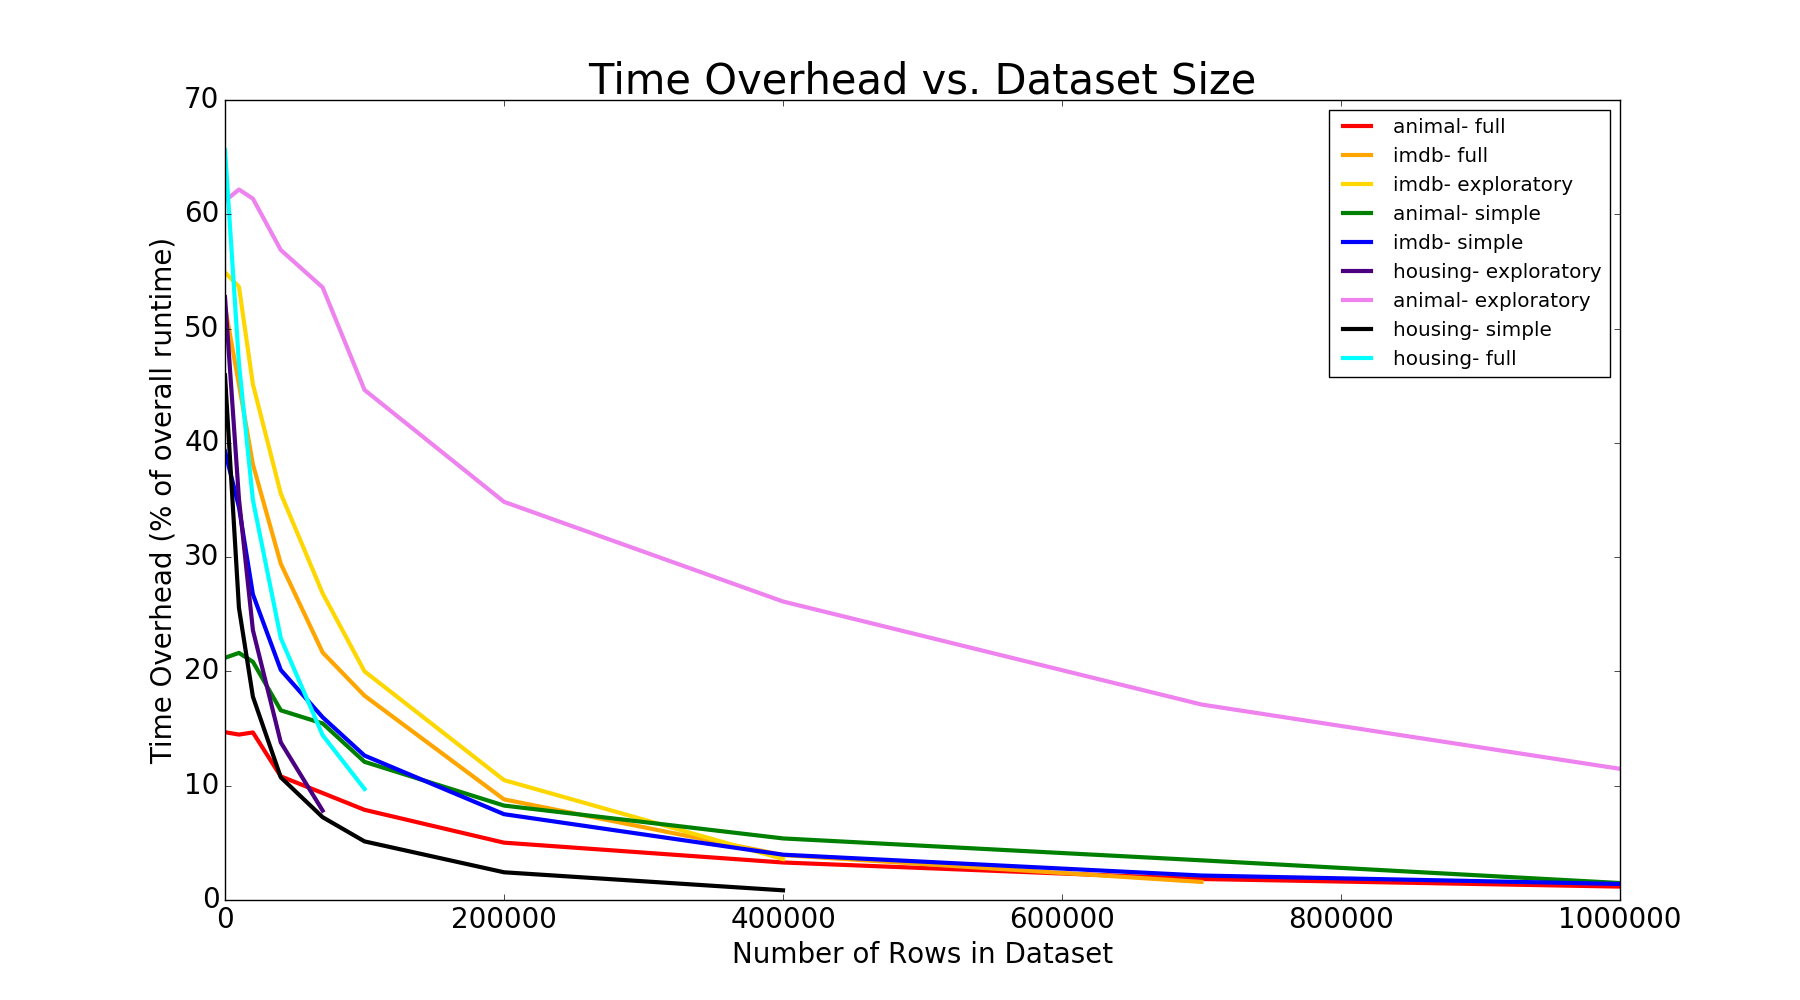
\includegraphics[width=6.0in]{time_overhead}
  \caption{
    Time overhead of ModelDB S+C.
  }
  \label{fig:time_overhead}
\end{figure}

Figure \ref{fig:time_overhead} shows that, as the dataset size grows, the time overhead
percentage for ModelDB S+C goes down. For a one million row dataset,
most of the workflows spend less than 5\% of their time running ModelDB S+C code.

For the results here, ModelDB S+C is configured not to count the number of rows in the DataFrames.
Counting the number of rows in a Spark DataFrame requires a sequential scan of the DataFrame. Doing this
would cause the absolute time spent running ModelDB S+C code to grow linearly with the dataset size. So, ModelDB Spark
Client disables row-counting by default.

In Figure \ref{fig:time_overhead}, the dataset size is measured in number of rows, rather than in
the actual size of the data file. This is done because the file format of the data has a big impact on
the size of the data file. Nevertheless, for reference, the largest dataset size (1 million rows) was under 300 MB
in size. All data was in CSV format.

Thus, Figure \ref{fig:time_overhead} shows that the time overhead of ModelDB S+C becomes insignificant 
as the dataset grows beyond 300 MB. 

The slowest step in recording and storing a model or operation, as determined by 
instrumenting various lines of code, is writing to the SQLite database. This is not a surprise
because the SQLite file lives on disk and because SQLite is not a very performant database.
Replacing SQLite with a more performant database may not only reduce the time overhead, it may
also reduce the storage requirements as well if data is appropriately compressed.

Focusing on the individual operations, the operation that consumed the most time, by far, was
GridSearchCrossValidationEvent. The average time overhead percentages for the most time
consuming operations are shown in Figure \ref{fig:event_time_overhead}.

\begin{figure}
  \centering
  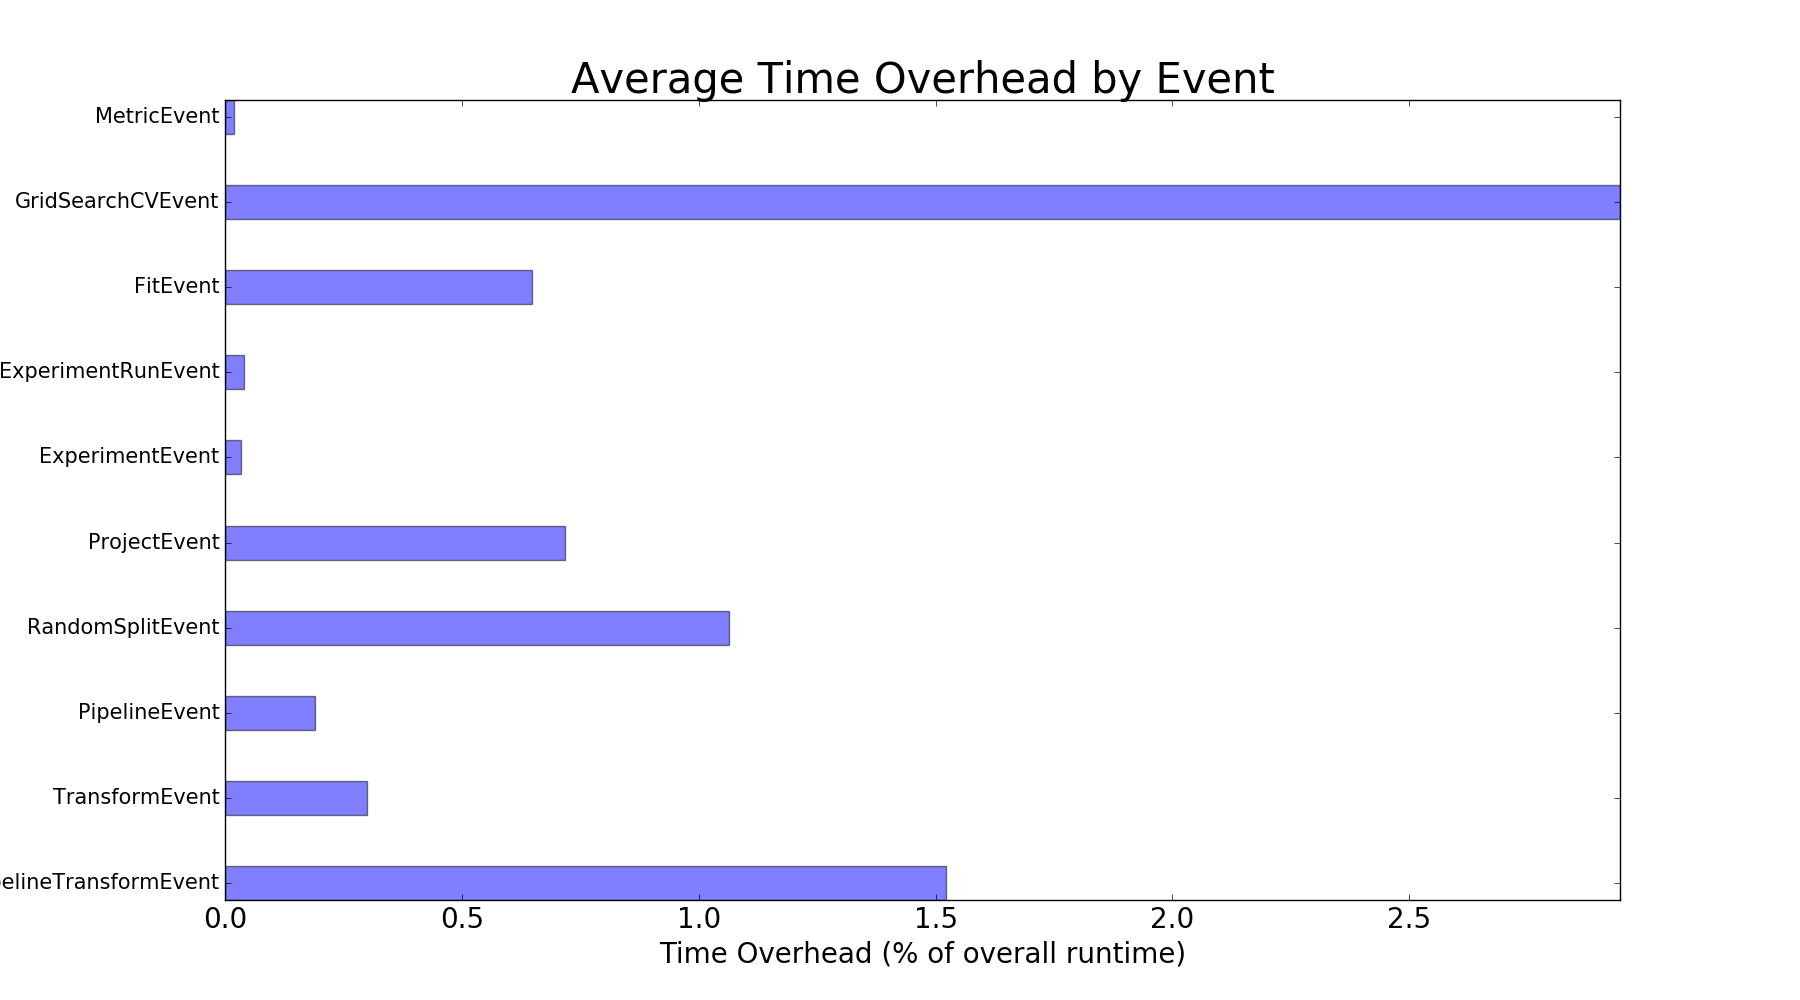
\includegraphics[width=6.0in]{event_time_overhead}
  \caption{
    Average time overhead percentage by event.
  }
  \label{fig:event_time_overhead}
\end{figure}

Figure \ref{fig:event_time_overhead} shows that roughly 3\% of the time in the overall
program is spent storing GridSearchCrossValidationEvents. This occurs because a GridSearchCrossValidationEvent
has many other smaller events contained inside it, such as TransformEvents, FitEvents, MetricEvents, and 
CrossValidationEvents. Consequently, ModelDB Server has to write many rows to many database tables when a
GridSearchCrossValidationEvent occurs. If the user is not interested in storing all the intermediate FitEvents,
TransformEvents, etc. for a GridSearchCrossValidation, then much of this overhead is a waste. Therefore, ModelDB S+C
allows the user to configure whether they would like to actually store all the data associated with a GridSearchCrossValidationEvent,
or whether they would like to simply store the FitEvent associated with the produced model. This makes it possible to cut out
much of the overhead caused by GridSearchCrossValidationEvents.

Thus, to summarize, ModelDB S+C's time overhead is small when the dataset is large (i.e. 300 MB or more). A
large fraction of the time is spent storing GridSearchCrossValidationEvents, and since the user may not
care about storing all the intermediate TransformEvents, MetricEvents, etc., the user is allowed to indicate 
whether they would like to store the full event or or just the FitEvent for the produced model.

\section{Storage Overhead Results}
For a fixed (dataset, workflow) pair, the size of ModelDB S+C's database and the size of the
model files do not change even as the number of rows in the dataset changes. This makes sense
because, except for counting the number of rows, ModelDB S+C does not access any data from the
DataFrame's rows. The size of ModelDB S+C's SQLite database is shown for each of the (dataset, workflow)
pairs in Figure \ref{fig:dbsize}.

\begin{figure}
  \centering
  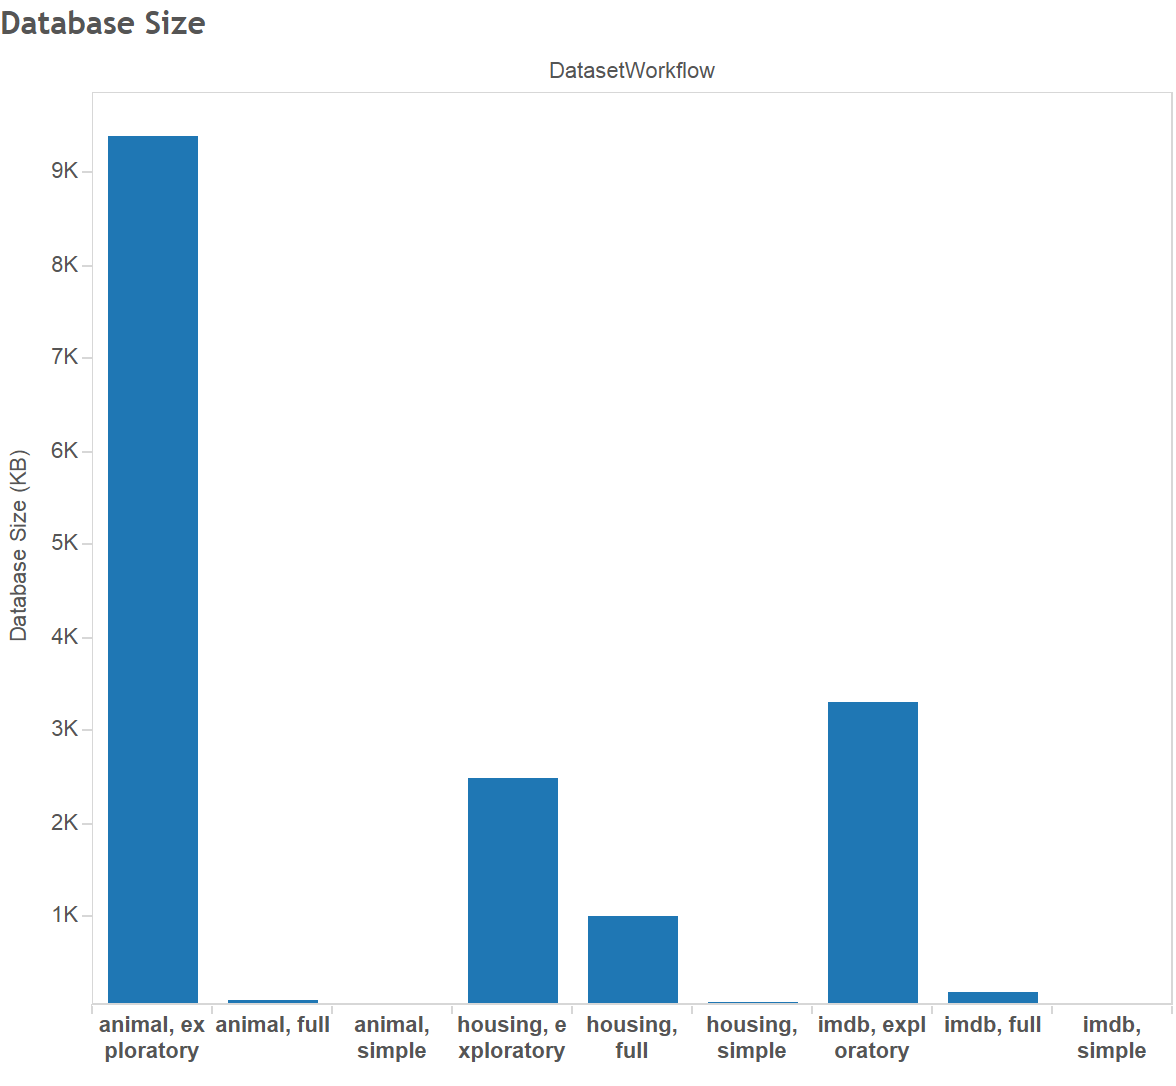
\includegraphics[height=4.0in]{dbsize}
  \caption{
    Database size (in KB) for each (dataset, workflow) pair.
  }
  \label{fig:dbsize}
\end{figure}

For all the (dataset, workflow) pairs, the database size remains under 10MB, and is
just a few MB for most of the (dataset, workflow) pairs. Since machine learning datasets
tend to be large (e.g. several hundred GB), 10MB is quite small. That being said, inspecting
the number of rows in each table for the Animal Shelter exploratory workflow 
can provide some insight into reducing the database size even further. This is shown in Figure
\ref{fig:animal_exploratory_table_sizes}.

\begin{figure}
  \centering
  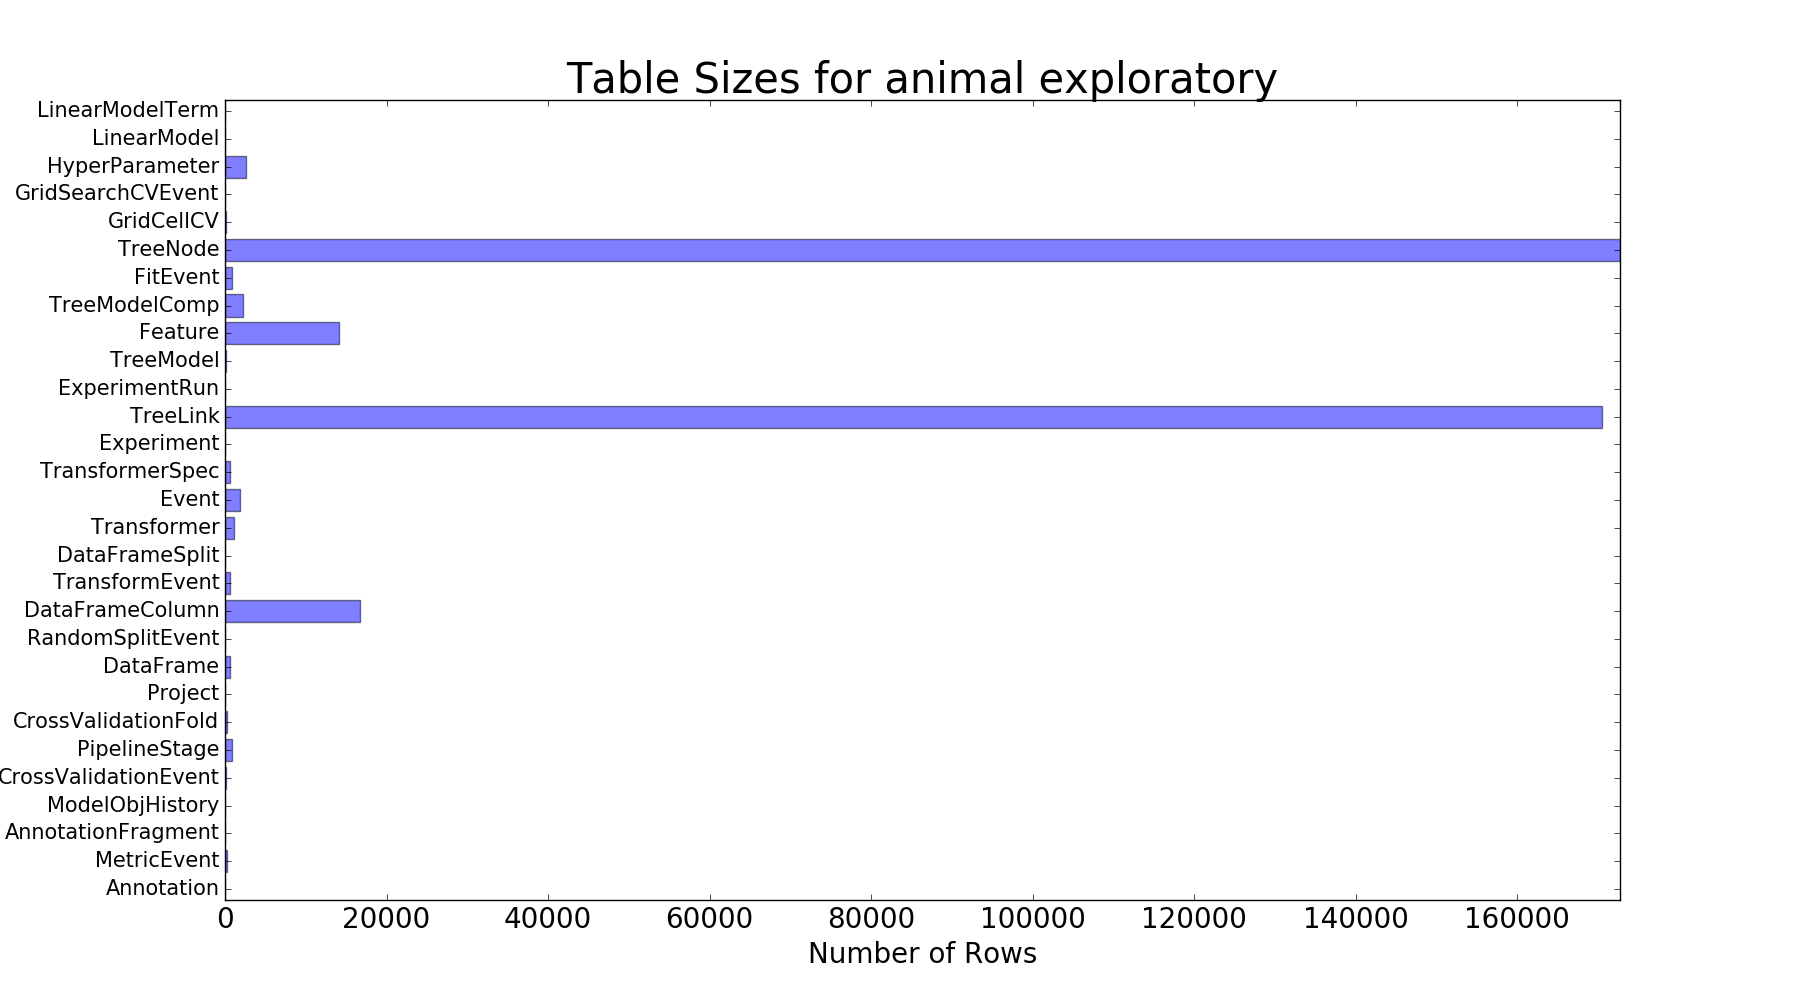
\includegraphics[width=6.0in]{animal_exploratory_table_sizes}
  \caption{
    Size of tables (in number of rows) for exploratory workflow for Animal
    Shelter dataset.
  }
  \label{fig:animal_exploratory_table_sizes}
\end{figure}

Overwhelmingly, the TreeModel and TreeLink tables have the most rows. A little
thought, however, shows that this is not surprising. The Animal Shelter exploratory workflow
trains a number of random forest models. Consider
a random forest with 20 decision trees where each tree has depth 7. Further assume
that each decision tree is a binary tree. This means that each tree has on the
order of $2^{7} = 128$ nodes (and roughly the same number of links). Thus, the
random forest has $20 \times 128 = 2560$ nodes (and roughly the same number of links).
If 3-fold grid search cross validation is conducted with 8 hyperparameter configurations (a $4 \times 2$ 
search grid), and a total of 3 such grid search cross validations are performed, 
this becomes $2560 \times 8 \times 3 \times 3 = 184,320$ nodes (and roughly the same number of links).
Therefore, it is no surprise that the TreeNode and TreeLink tables are so large.

ModelDB S+C provides two mechanisms to reduce database size. First, as described before, it
allows the user to forgo storing ALL the data associated with a GridSearchCrossValidationEvent and instead
store only the most important parts.
Second, it allows the user to forgo storing entries in the TreeLink and TreeNode table (the
node and link data are already stored in the serialized model file) except for specified models. This can reduce the database size
greatly, and allow the user to only store TreeNode and TreeLink rows when it is necessary. In the 
exploratory workflow for the Animal Shelter workflow, only one (i.e. the best)  model's TreeLink and TreeNode data is really needed,
but the workflow stores data for dozens of random forest models. When the above two mechanisms are applied,
the size of the database falls from about 9 MB to 1.6 MB, as shown in figure \ref{fig:dbsize_small}.

\begin{figure}
  \centering
  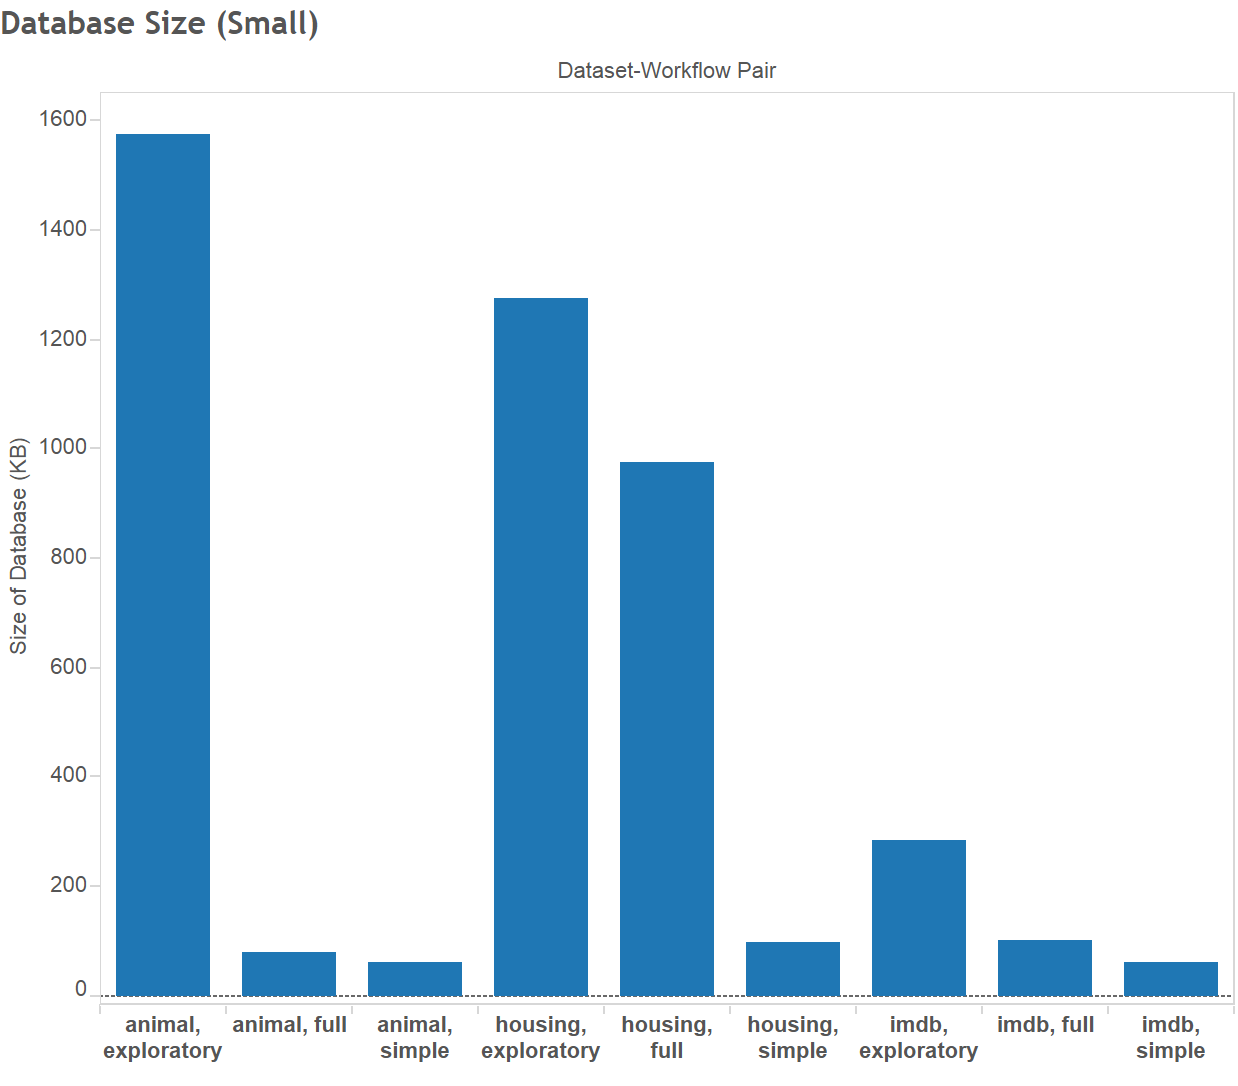
\includegraphics[width=5.0in]{dbsize_small}
  \caption{
    Size of database for each (dataset, workflow) pair when GridSearchCrossValidationEvent intermediates
    are not stored and when the TreeLink and TreeNode tables are only populated for the last model.
  }
  \label{fig:dbsize_small}
\end{figure}


Finally, it is worth looking at the size of the model files produced by each (dataset, workflow) pair. This is shown in
Figure \ref{fig:modelsizes}.

\begin{figure}
  \centering
  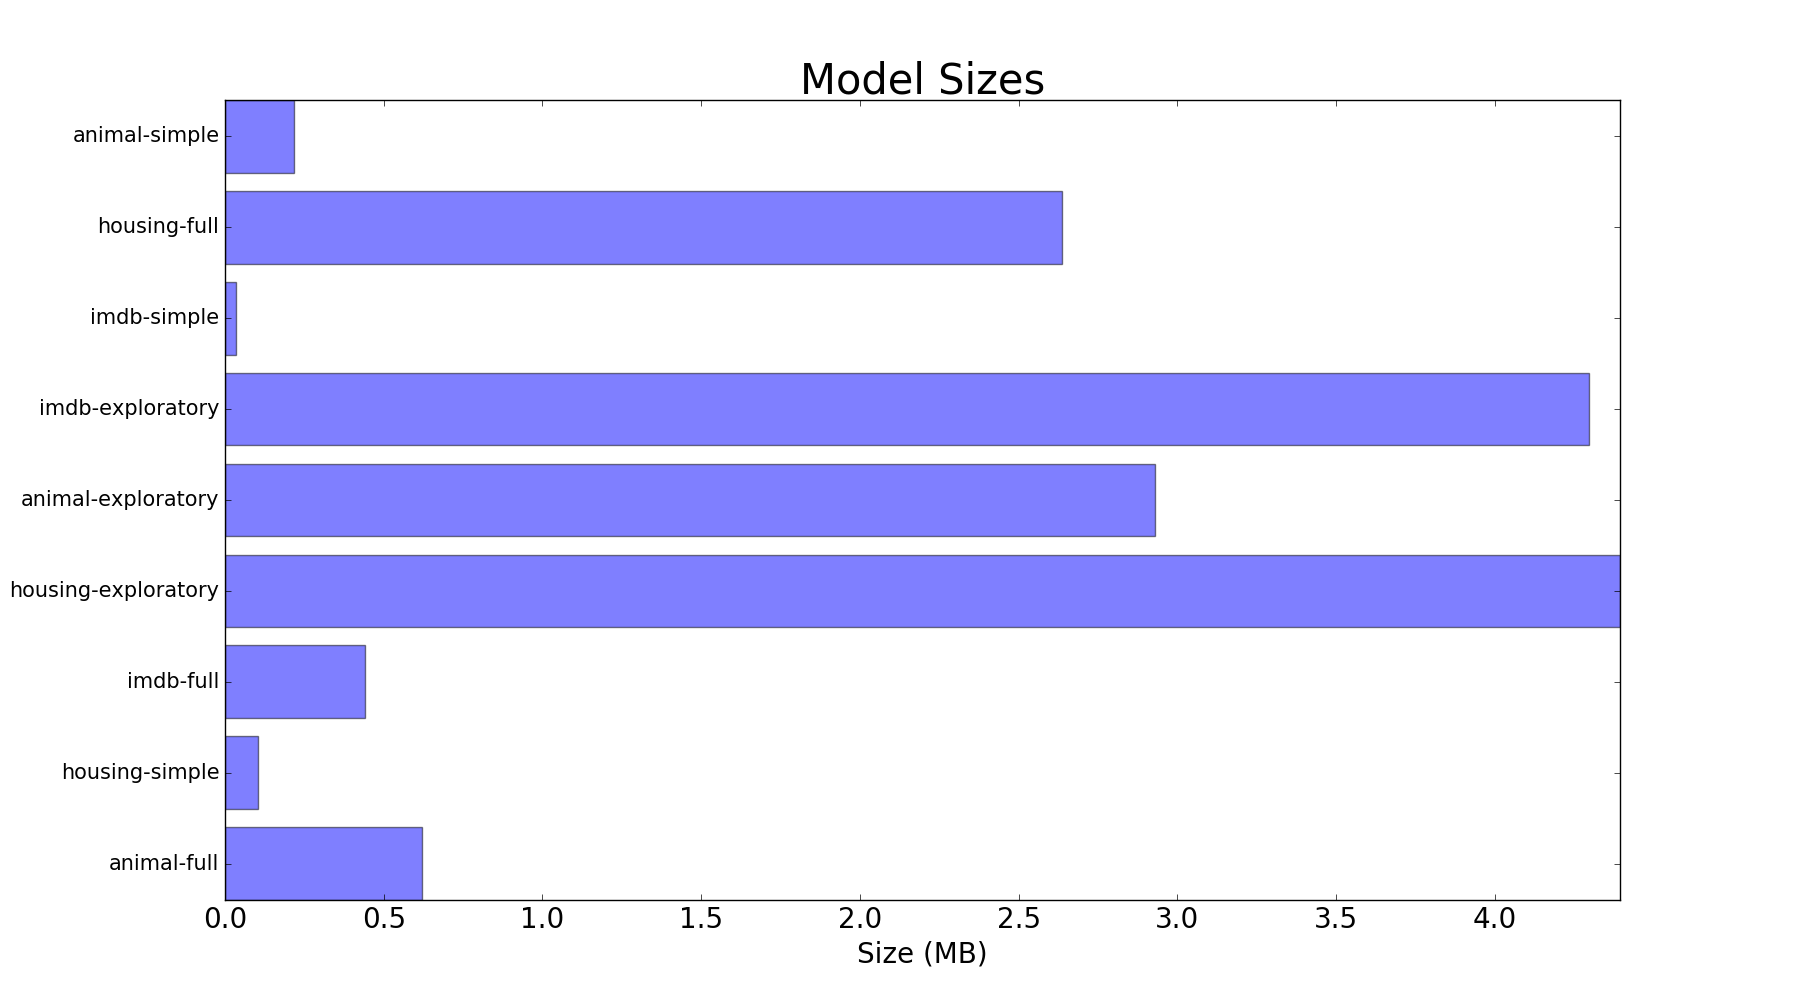
\includegraphics[width=5.0in]{modelsizes}
  \caption{
    Size of model files for each (dataset, workflow) pair.
  }
  \label{fig:modelsizes}
\end{figure}

Again, while these sizes are small (< 5 MB) compared to the size of typical machine learning
datasets, they can still be reduced. Rather than serializing and storing every single model produced in the 
workflow, ModelDB S+C allows the user to indicate which models they would actually like to serialize and store (by
calling saveSync() on the model). When the final models are explicitly serialized and stored, rather than serializing and storing
all the produced Transformers, the model sizes in Figure \ref{fig:modelsizes_small} occur. 

\begin{figure}
  \centering
  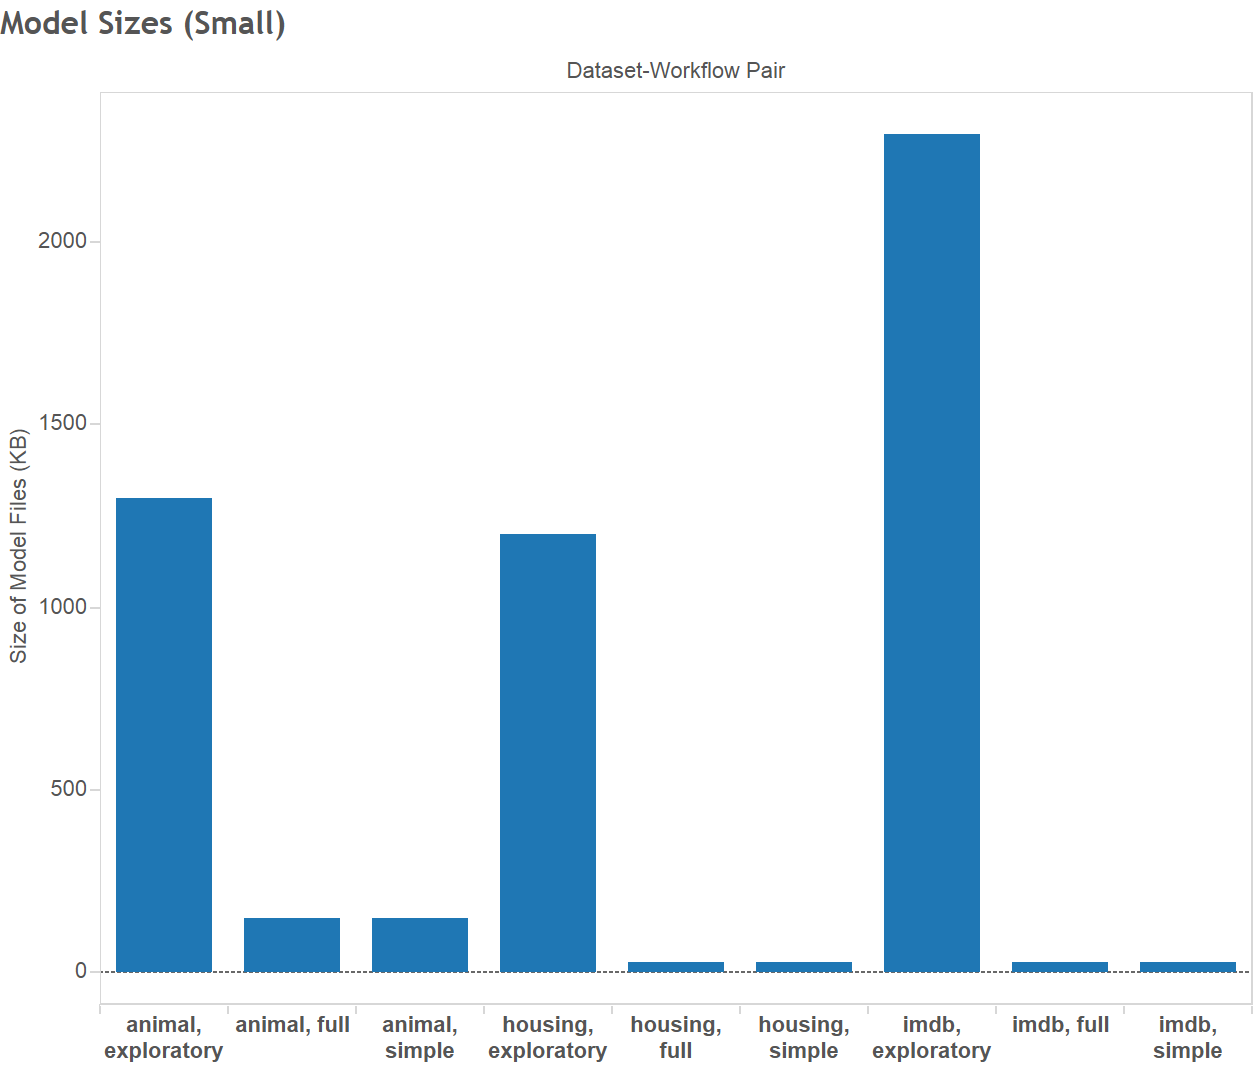
\includegraphics[width=5.0in]{modelsizes_small}
  \caption{
    Size of model files for each (dataset, workflow) pair when only the final models are serialized
    and stored, rather than serializing and storing all produced Transformers.
  }
  \label{fig:modelsizes_small}
\end{figure}

The models in Figure \ref{fig:modelsizes_small} take up much less space.

\section{API Method Time Results}
The IMDB exploratory workflow took about 490 seconds (a little over 8 minutes)
to execute, and the majority of this time was spent training models. Figure \ref{fig:methodtimes}
shows the time taken by various API method, as a function of the number of times each row
was duplicated (recall that the duplication was done to simulate multiple workflows).

\begin{figure}
  \centering
  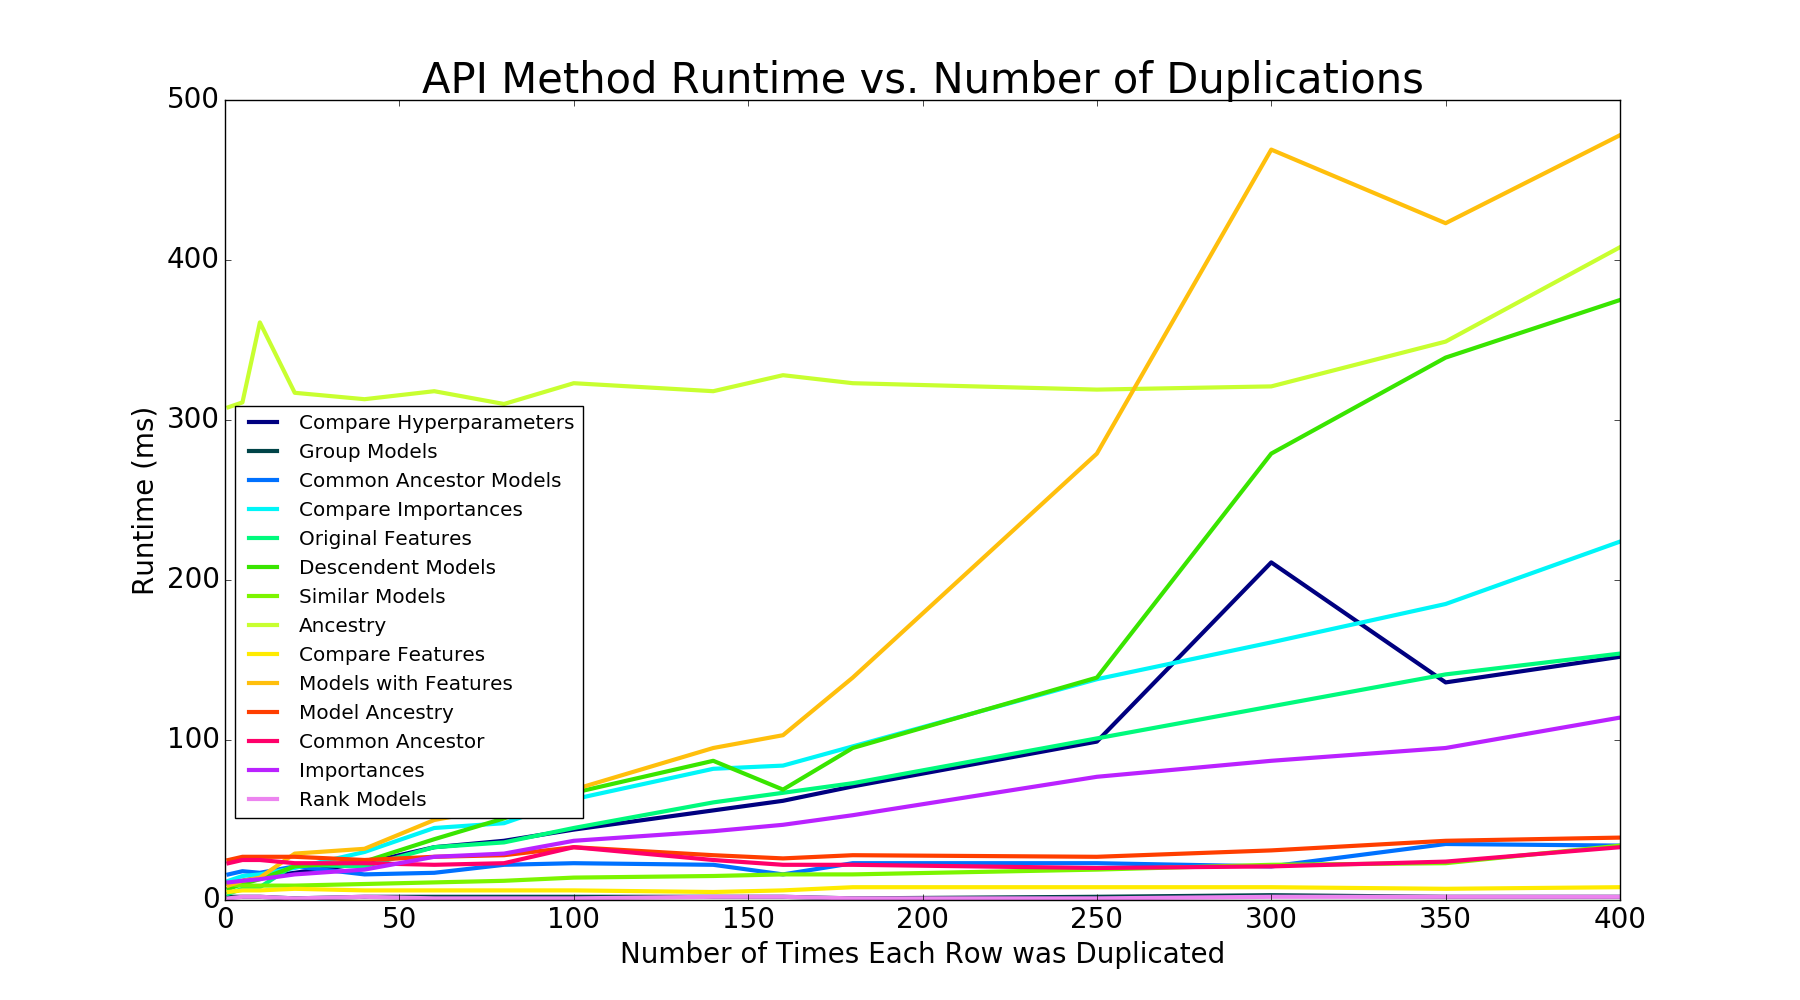
\includegraphics[width=6.0in]{methodtimes}
  \caption{
    Time taken for each method, plotted as a function of the number of times that
    each row was duplicated.
  }
  \label{fig:methodtimes}
\end{figure}

Figure \ref{fig:methodtimes} shows that the running times of the API methods are
very small, with not a single API method taking more than 500 milliseconds. The fast running
times are due to the indices in ModelDB Server's database, which speed up the slow queries
and due to the fact that all of ModelDB Server's API methods run in $O(n)$ time or better, where
$n$ is the size of the database. The running time grows slowly with the number of workflows, and
should remain small (under a few seconds) even for a large number of workflows. That being said, there are still
a few potential indices that could be created in order to speed up the API methods. Second, some API
methods (e.g. descendent models) could theoretically be parallelized. Third, the overall ModelDB system includes
abstractions for grouping together Syncable Events and primitives (e.g. ExperimentRun, Project), and queries could be
restricted to run within a specific ExperimentRun or Project, because these tend to be small. Fourth,
using a more performant database than SQLite could speed up the API methods. Overall, though, the running
time of the API methods is very small compared to the time taken to run the IMDB exploratory workflow.

\section{Model Files Compared to PMML Results}
The PMML Website includes model files for a random forest model and logistic regression
model training on the Iris dataset. To compare ModelDB S+C's storage to PMML, a
a random forest model and one vs. rest logistic regression model were trained on the Iris
dataset. The results are shown in Table \ref{tab:pmml}. Note that the one vs. rest classifier
actually trains multiple logistic regression models. A one vs. rest classifier was used
because Spark.ML does not currently support the multi-class logistic regression model. To
compensate, only one logistic regression model is counted for the sizing, rather than
all of them.

 \begin{table}
   \centering
    \begin{tabular}{ | l | l | l | l |}
      \hline
      Model Type & Database Size (KB) & Models Size (KB) & PMML Size (KB) \\ \hline
      Logistic Regression & 16 & 12 & 4 \\ \hline
      Random Forest & 116 & 224 & 420 \\ 
      \hline
   \end{tabular}
   \caption{Comparing ModelDB database and model files to PMML file}
   \label{tab:pmml}
 \end{table}

 So, for the logistic regression model, ModelDB S+C uses $16 + 12 = 28$ KB, which is
 higher than the $4$ KB required for PMML. This is because the logistic regression model
 is quite simple, which allows the PMML file to be small. ModelDB S+C must store information
 about the DataFrame, TransformerSpec, DataFrameColumns, and Hyperparameters in its database and
 it stores some metadata for the deserializer in the model file. These two factors cause ModelDB S+C
 to use more storage space than the PMML file does.

 The situation is reversed for the random forest, however. ModelDB S+C only uses $116 + 224 = 340$ KB,
 while the PMML file uses $420$ KB. The random forest is large (200 trees), so the overhead of storing the DataFrame,
 TransformerSpec, DataFrameColumn, and Hyperparameters and the overhead of storing deserialization metadata are now small.
 ModelDB is able to leverage the (somewhat) efficient storage format of SQLite and efficient storage format of Parquet (for 
 the model file), which keeps the overall storage space small. PMML, on the other hand, is an XML-like language, which becomes
 quite verbose for a large model like the random forest.

 Overall, it seems that ModelDB S+C does not require significantly more storage space than PMML for storing models. 
 While it may require more storage space in some cases, it is worth it because PMML cannot be queried like the SQLite
 database can and Spark.ML cannot deserialize PMML models and use them in the program. One advantage that PMML
 has is that it is a human readable file (The Parquet file and SQLite file are not human readable) and it is more well-known. 
 However, since ModelDB S+C is not tied to a particular storage format, the user could store their serialized model in PMML, 
 if they so choose.

\section{Evaluating Existing Workflows Results}
Three real machine learning workflows (Flight Delays, Titanic, and SMS Spam) were
considered and modified to use ModelDB S+C. This was done to see how many operations in the
machine learning workflow ModelDB S+C is able to record. Note in the following paragraphs that "captures"
means that ModelDB S+C is able to automatically record and store the operations and machine learning models
associated with a step of the workflow.

The Flight Delays workflow begins by reading the CSV file and parsing the data. These parsing
steps (e.g. convert timestamp into Java Date) are not captured by ModelDB S+C. While it is possible
for the user to indicate this parsing step by manually buffering a TransformEvent in the ModelDBSyncer,
it is not done automatically. Then, the workflow creates a pre-processing pipeline, which can be captured
completely by ModelDB S+C. Next, a decision tree model and logistic regression model are trained and
used to make predictions on the test data - this too can be captured completely by ModelDB S+C.

The Titanic workflow begins by reading the data and splitting the data into training and testing sets, which is captured by
ModelDB S+C. Then, it creates a number of visualizations - this is completely ignored by ModelDB S+C.
Next, some null values are are replaced with the median value of the column - this is not automatically 
captured by ModelDB S+C, but the user could manually log a TransformEvent to indicate this cleaning step.
Then, grid search cross validation is used to train a logistic regression model - ModelDB S+C completely 
captures this step. Next, a random forest model is trained using grid search cross validation, and this too
is completely captured by ModelDB S+C. Then, the feature importances of the models are listed - this too
is captured by ModelDB S+C (it stores feature importances for linear and tree models).

The SMS Spam workflow begins by reading the data and applying a HashingTF transformer to it - ModelDB S+C
can capture this step. Then, a logistic regression mdoel is trained, which ModelDB S+C captures. Finally,
the model is used to make some predictions, which is also captured by ModelDB S+C.

The above examples illustrate that ModelDB S+C is able to log many of the machine learning operations and 
models in actual machine learning workflows. It is not able to log any created visualizations, but that is out
of scope for ModelDB S+C. There are some data parsing and cleaning steps that it is not able to log automatically, but
it allows the user to manually buffer a TransformEvent for this purpose. In the case of the workflows above, it
may actually be possible to log some of the data parsing and cleaning steps automatically (create implicit classes for
Spark's RDD methods and log a TransformEvent when they are executed), but that has not been
implemented yet in ModelDB Spark Client.

\section{Improvements}
While a number of potential improvements have been discussed in the previous sections,
it is worth focusing on a few of them below.

First, using a better database than SQLite may improve ModelDB S+C's storage and time
overhead. SQLite is not designed for performance. It was used because it is simple and allows
ModelDB S+C to be used out of the box.

Second, ModelDB S+C misses a number of opportunities to parallelize queries. For example,
when storing CrossValidationEvents in a GridSearchCrossValidationEvent, each CrossValidationEvent
is stored one at a time. This is not strictly necessary, as they could be stored in parallel.
Writing ModelDB's storage algorithms so that they can store multiple Syncable Events or primitives 
in parallel may speed up the runtime significantly.

Third, rather than creating a TreeLink table and TreeNode table, it may be possible to store
tree models in a JSON column. Since JSON columns are not supported in SQLite, however, this was
not done.

Fourth, ModelDB does not apply any compression of its model files. Doing this can reduce their storage requirements.

\chapter{Role in Overall ModelDB System}
ModelDB S+C was not built in isolation. It interacts with a number of other
systems in an overall system called ModelDB. ModelDB is a system for machine learning
model management. It includes:

\begin{enumerate}
\item a web application for visualizing and examining data about models and operations
\item a client, like the Spark Client, designed for Python's Scikit-learn machine learning
library
\item a command line toolkit that includes a versioning system for code
\item a prediction store for the predictions made by models
\end{enumerate}

Figure \ref{fig:system_architecture} showed the system architecture
of ModelDB S+C. Figure \ref{fig:full_system_architecture} augments Figure \ref{fig:system_architecture}
to show how some of the other pieces of ModelDB interact with ModelDB S+C. The prediction store
is excluded from the figure because it currently has not been integrated into the rest of the ModelDB
system.

\begin{figure}
  \centering
  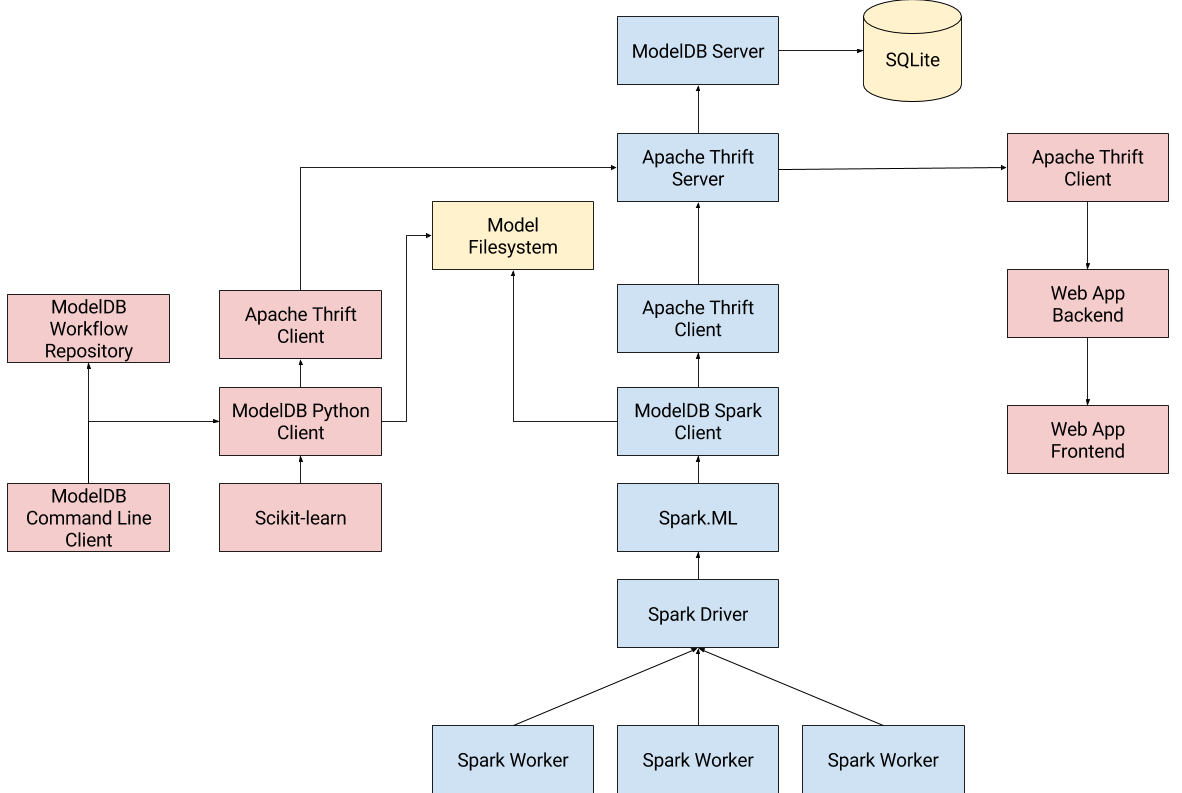
\includegraphics[height=4.0in]{full_system_architecture}
  \caption{
    The overall architecture of ModelDB that shows the components
    that interact with ModelDB S+C. The arrows indicates the flow
    of operations + models data. 
  }
  \label{fig:full_system_architecture}
\end{figure}

The other systems in ModelDB can be seen as use cases that demonstrate how ModelDB S+C
can serve as a foundation for other applications.

\section{Scikit-learn Client}
ModelDB includes a client for Python's Scikit-learn machine learning library. Like the
ModelDB Spark Client, the Scikit-learn Client also utilizes the ModelDB Syncer abstraction,
the Syncable Event abstraction, and the "Sync" API (e.g. fitSync, transformSync). This Scikit-learn
Client was inspired by the abstractions in ModelDB Spark Client, and demonstrates that the ModelDB Server
abstractions (e.g. FitEvent, TransformerSpec) can generalize to other machine learning libraries and that
ModelDB Spark Client abstractions (e.g. ModelDBSyncer) can also generalize to other machine learning libraries.

\section{Command Line Toolkit}
ModelDB includes a command line toolkit that allows users to record various operations (e.g.
evaluation of a model) without using any kind of machine learning library. This command line toolkit still
uses the underlying abstractions in ModelDB Server, showing that they can generalize even if there is no machine learning
library.

\section{Web Application}
ModelDB includes a web application that can display information about models and visualizations of
the model building process. This web application is built directly on the API methods exposed by the ModelDB Server,
and does not actually use the database directly. This shows how an application can be built on top of ModelDB Server's 
data and API.

\section{Possible Database Applications}
Although no applications in ModelDB access the database directly, the database, on its own, 
serve as a building block for other applications. Additionally, the database could simply be used in other data management
systems, like DataHub \cite{datahub}.

\chapter{Future Work}

\chapter{Conclusion}

\appendix
\chapter{Tables}

\begin{table}
\caption{Armadillos}
\label{arm:table}
\begin{center}
\begin{tabular}{||l|l||}\hline
Armadillos & are \\\hline
our	   & friends \\\hline
\end{tabular}
\end{center}
\end{table}

\clearpage
\newpage

%\chapter{Figures}

\vspace*{-3in}

\begin{figure}
\vspace{2.4in}
\caption{Armadillo slaying lawyer.}
\label{arm:fig1}
\end{figure}
\clearpage
\newpage

\begin{figure}
\vspace{2.4in}
\caption{Armadillo eradicating national debt.}
\label{arm:fig2}
\end{figure}
\clearpage
\newpage

%% This defines the bibliography file (main.bib) and the bibliography style.
%% If you want to create a bibliography file by hand, change the contents of
%% this file to a `thebibliography' environment.  For more information 
%% see section 4.3 of the LaTeX manual.
\begin{singlespace}
\bibliography{main}
\bibliographystyle{plain}
\end{singlespace}

\end{document}

